%!TEX program = xelatex
\documentclass[10pt, compress]{beamer}
\usetheme[titleprogressbar]{m}

\usepackage{booktabs}
\usepackage[scale=2]{ccicons}
\usepackage{minted}
\usepackage{comment}
\usepackage{csquotes}
\usepackage[backend=biber,style=authoryear]{biblatex}
\usepackage[main=german]{babel}
\usepackage{amsmath}
\usepackage{amssymb}
\usepackage{amsfonts}
\usepackage{caption}
\usepackage{subcaption}
\usepackage{tikz}
\usepackage{pgfplots}
\pgfplotsset{every axis/.append style={very thick}}
\usefonttheme[onlymath]{serif}

\renewcommand*{\nameyeardelim}{\addcomma\space} 
\usepgfplotslibrary{dateplot}
\usemintedstyle{trac}

\setbeamertemplate{section in toc}{\inserttocsectionnumber.~\inserttocsection}
\setbeamercolor{section in toc}{fg=black}

\addbibresource{references.bib}

\title{Data Augmentation mit Variational Autoencodern}
\date{\today}
\author{Henri Iser}
\institute{Rheinische Friedrich-Wilhelms-Universität Bonn}


\begin{document}
\maketitle

\begin{frame}{Gliederung}
  \tableofcontents
\end{frame}


\section{Motivation}
\begin{frame}{Motivation}
  \begin{itemize}
    \item Neuronale Netzwerke lösen komplexe Aufgaben
    \item Anforderung der großen Datenmengen oft nicht erfüllbar (\textit{Few-Shot Learning})\\
    $\Rightarrow$ Data-Augmentation
    \item Generative Modelle effizient
    \item \textbf{Hier} Variational Autoencoder als Data Augmentation Ansatz
  \end{itemize}
\end{frame}


\section{Variational Autoencoder}
\begin{frame}{Autoencoder}
  \begin{figure}[hbt]
    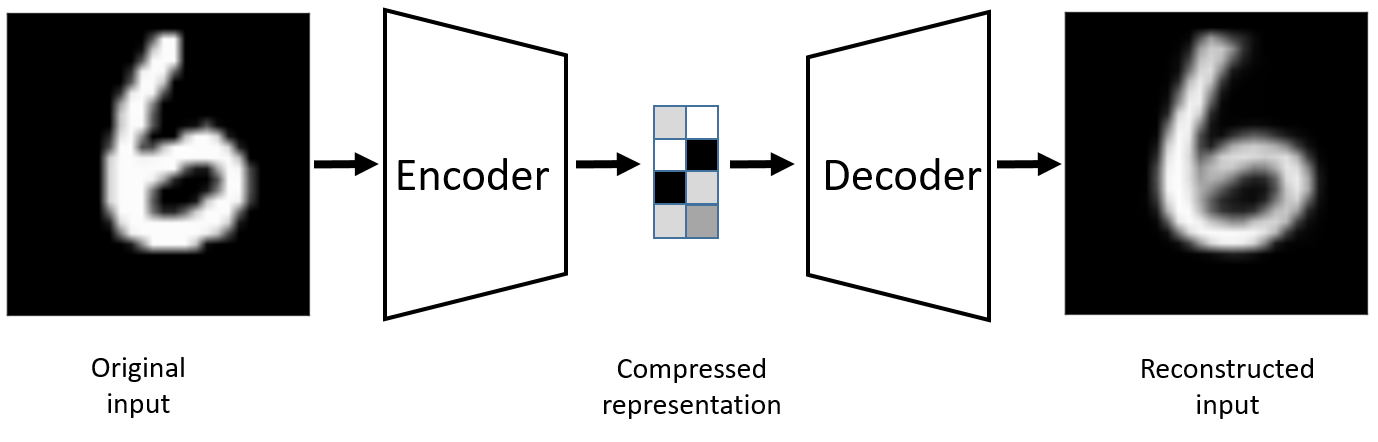
\includegraphics[width=.5\textwidth]{gfx/literature/autoencoder}
    \caption{Encoder-Decoder Architektur$^1$}
  \end{figure}
  \begin{itemize}
    \item Merkmalsvektoren stellen Repräsentation der Eingabe dar
    \item Merkmalsraum hat keine geometrische Struktur
  \end{itemize}
  \vfill
  {\tiny $^1$ entnommen aus \cite{LopezPinaya2019}}
\end{frame}

\begin{frame}{Variational Autoencoder}
  \begin{minipage}[c]{.5\textwidth}
    \begin{figure}[hbt]
      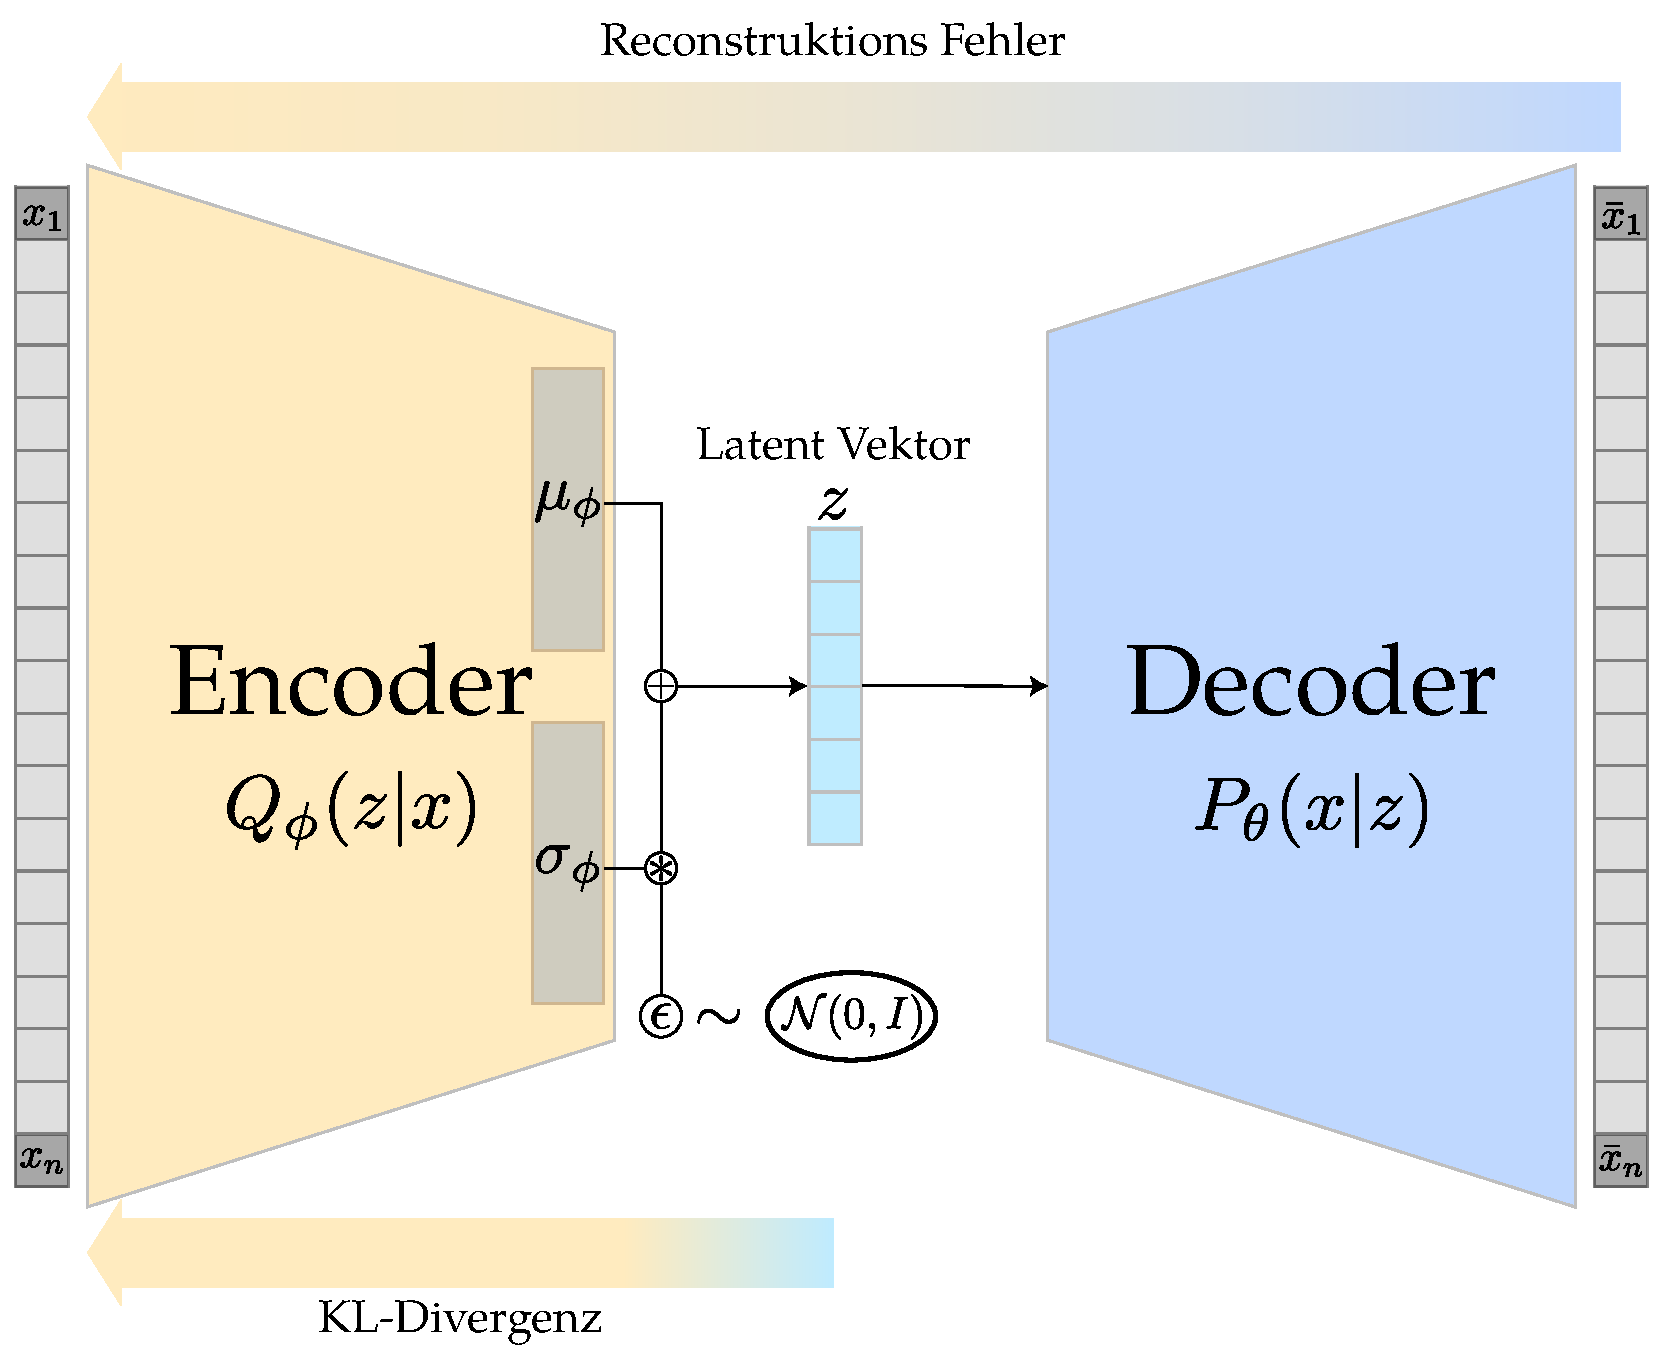
\includegraphics[width=\textwidth]{gfx/literature/VAE Architecture}
      \caption{VAE Architektur}
    \end{figure}
  \end{minipage}
  \hfill
  \begin{minipage}[c]{.45\textwidth}
    Rekonstruktions Fehler
    \begin{equation*}
      \mathcal{L}_{NLL} = - \mathbb{E}_{z \sim Q_\phi(z, \vert x)} \left[ \log P_\theta(x \vert z) \right]
    \end{equation*}
    \\
    KL-Divergenz
    \begin{equation*}
      \mathcal{L}_{KL} = \mathcal{D}_{KL}\left[ Q_\phi(x \vert z) \| \mathcal{N}(0, I) \right]
    \end{equation*}
  \end{minipage}
\end{frame}

\begin{frame}{$\beta$-VAE$^1$}
  \begin{equation}
    \mathcal{L}_{VAE} = \underbrace{\mathbb{E}_z \left[ \log P_\theta(x \vert z)\right]}_{\text{Rekonstruktionsfehler}} - \beta \cdot \underbrace{\mathbb{E}_z \left[ \mathcal{D}_{KL}\left[ Q_\phi(z \vert x) \| \mathcal{N}(0, I) \right] \right]}_{\text{KL-Divergenz}}
  \end{equation}
  \vfill
  außerdem
  \begin{equation}
    \beta_{norm} = \beta \cdot \frac{d}{N}, 
  \end{equation}
  mit Latent-Space Dimension $d$
  \vfill
{\tiny $^1$ vorgeschlagen von \cite{Higgins2017}}
\end{frame}

\begin{frame}{Variational Autoencoder}
  \begin{itemize}
    \item Merkmalsraum $\rightarrow$ Latent-Space
    \item Zwischenräume stellen Interpolationen dar
    \item Merkmale probabilistisch abgebildet
  \end{itemize}
  \vfill
  \begin{figure}[hbt]
  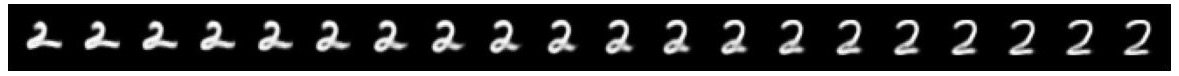
\includegraphics[width=\textwidth]{gfx/methodology/interpolation}
  \caption{Interpolation innerhalb der Klasse 2}
\end{figure}
\end{frame}


\section{Datensätze}
\begin{frame}{Datensätze}
\begin{minipage}[c]{.45\textwidth}
  \begin{figure}[b]
  \centering
  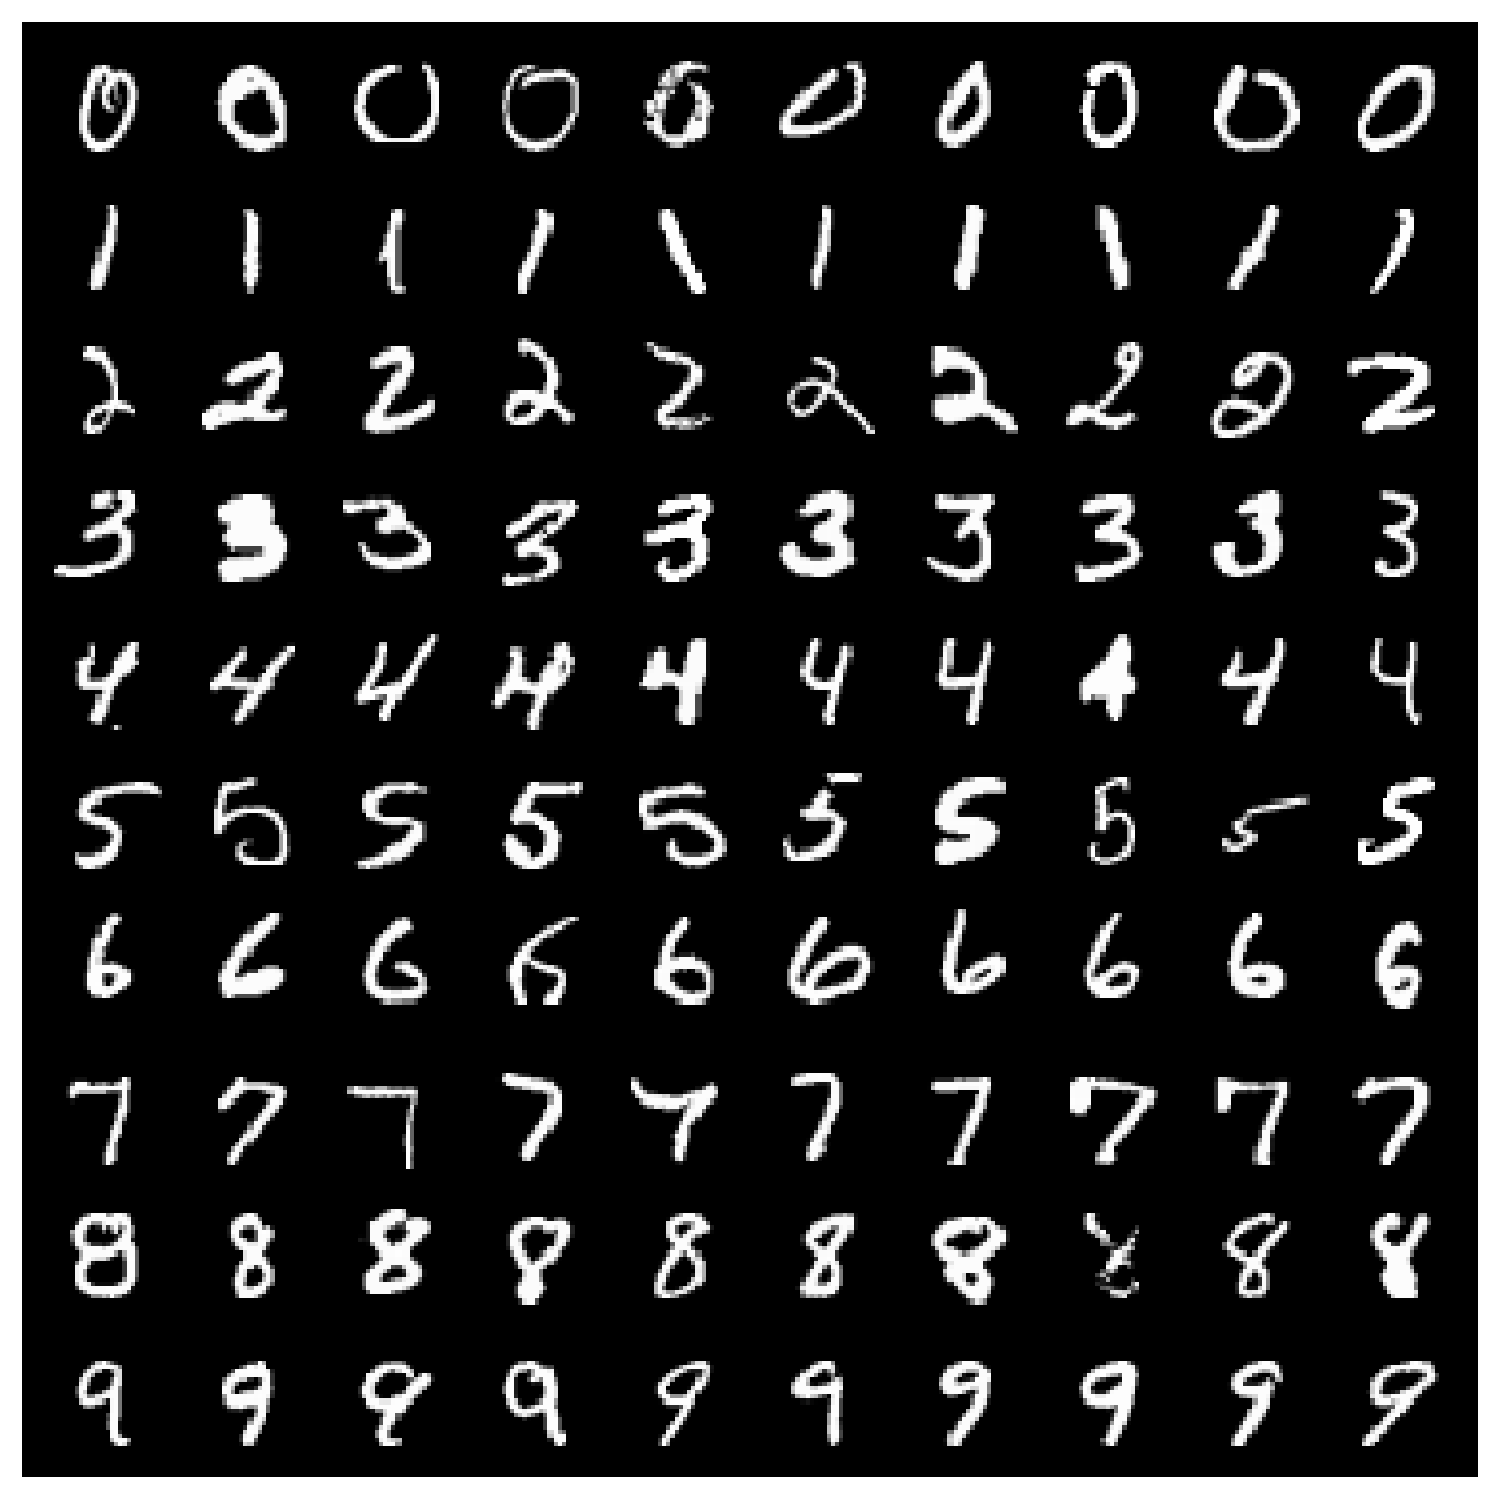
\includegraphics[width=\textwidth]{gfx/datasets/mnist_ciffers}
  \caption{MNIST Datensatz}
  \end{figure}
\end{minipage}
\hfill
\begin{minipage}[c]{.45\textwidth}
  \begin{figure}[b]
  \centering
  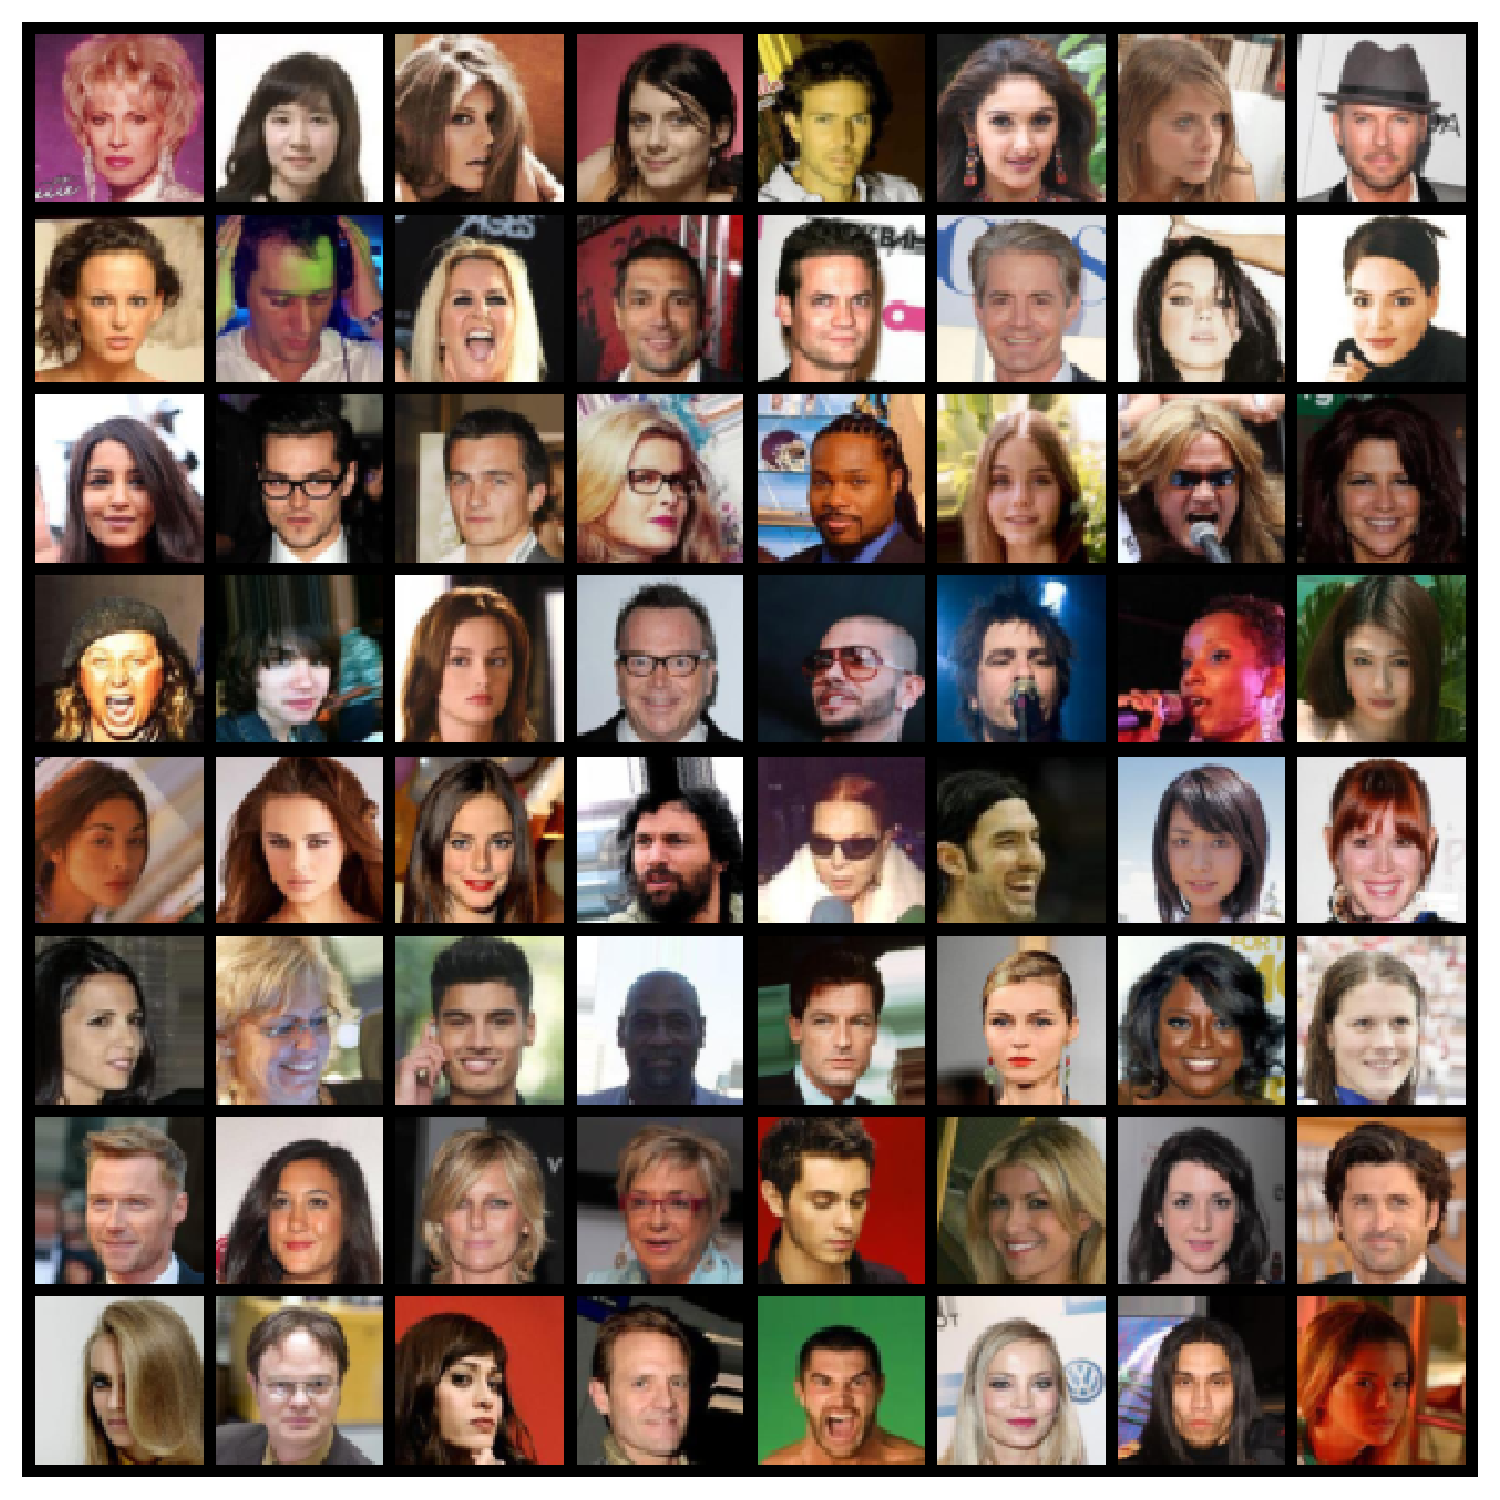
\includegraphics[width=\textwidth]{gfx/datasets/real}
  \caption{CelebA Datensatz}
\end{figure}
\end{minipage}
\end{frame}

\begin{frame}{Datensätze - PROBEN1}
  \begin{table}[hbt]
  \centering\scalebox{.7}{
  \begin{tabular}{l|l|l|l|l|l}
  \toprule
  Datensatz   & \# Attribute & kontinuierlich        & \# Klassen & \# Beispiele & Balancing \\ \hline
  card        & 15           & 0.40                  & 2          & 690          & 0.99      \\
  diabetes    & 8            & 1.00                  & 2          & 768          & 0.93      \\
  geneN       & 60           & 0.00                  & 3          & 3175         & 0.93      \\
  glass       & 9            & 1.00                  & 6          & 214          & 0.84      \\
  horse-colic & 20           & 0.70                  & 3          & 364          & 0.84      \\
  thyroid     & 21           & 0.29                  & 3          & 7200         & 0.28      \\
  \bottomrule
  \end{tabular}}
  \caption{PROBEN1 Datensatz Sammlung}
  \label{tab:PROBEN1-datasets}
  \end{table}
  \begin{itemize}
    \item numerische Attributsdaten
  \end{itemize}
\end{frame}


\section{Generieren neuer Beispiele}
\begin{frame}{Sampling im Latent-Space}
\begin{minipage}[c]{.39\textwidth}
\vspace*{1.1cm}
  \begin{figure}[hbt]
    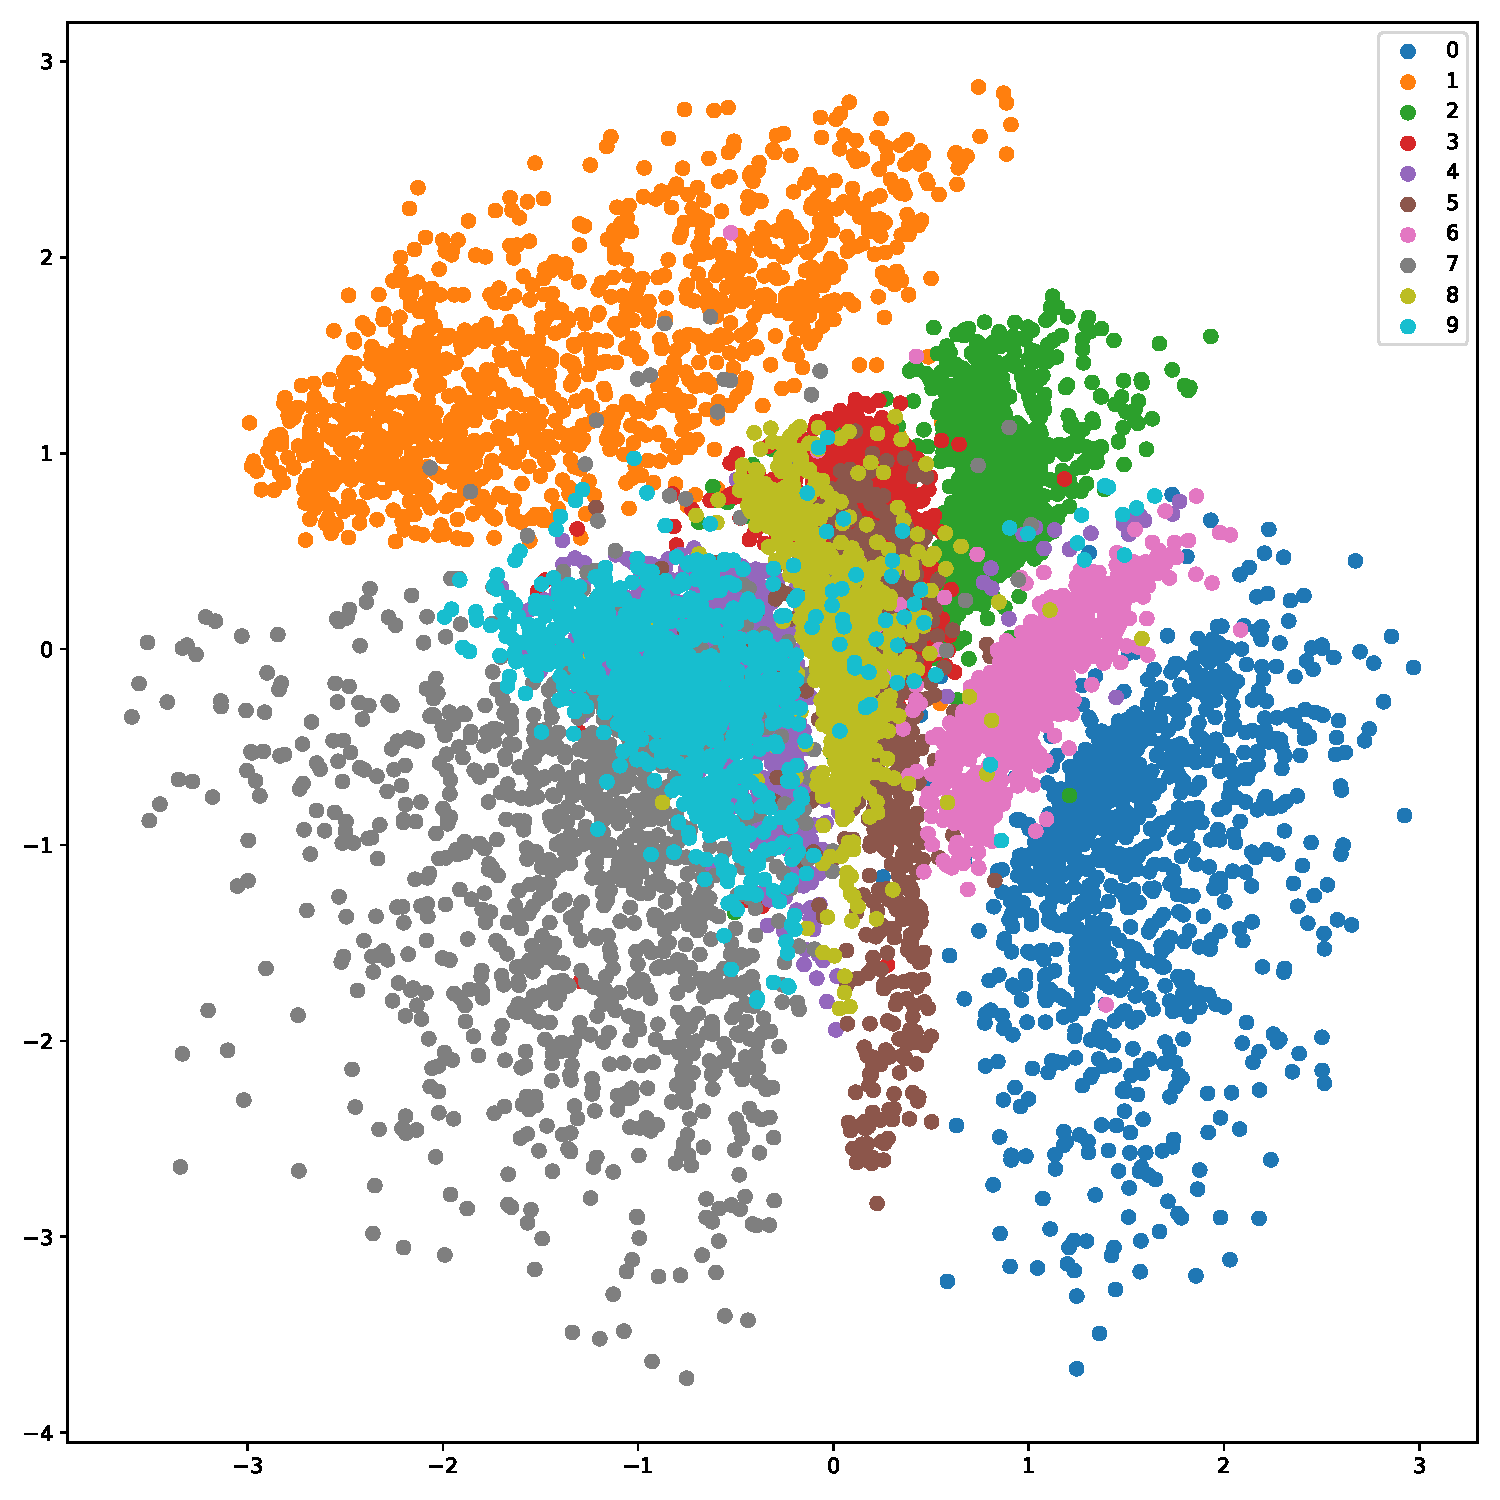
\includegraphics[width=\textwidth]{gfx/evaluation/feature_space/distributions_mnist}
    \caption{Latent-Space MNIST}
  \end{figure}
\end{minipage}
\hfill
$\Rightarrow$
\hfill
\begin{minipage}[c]{.5\textwidth}
  \begin{figure}[hbt]
    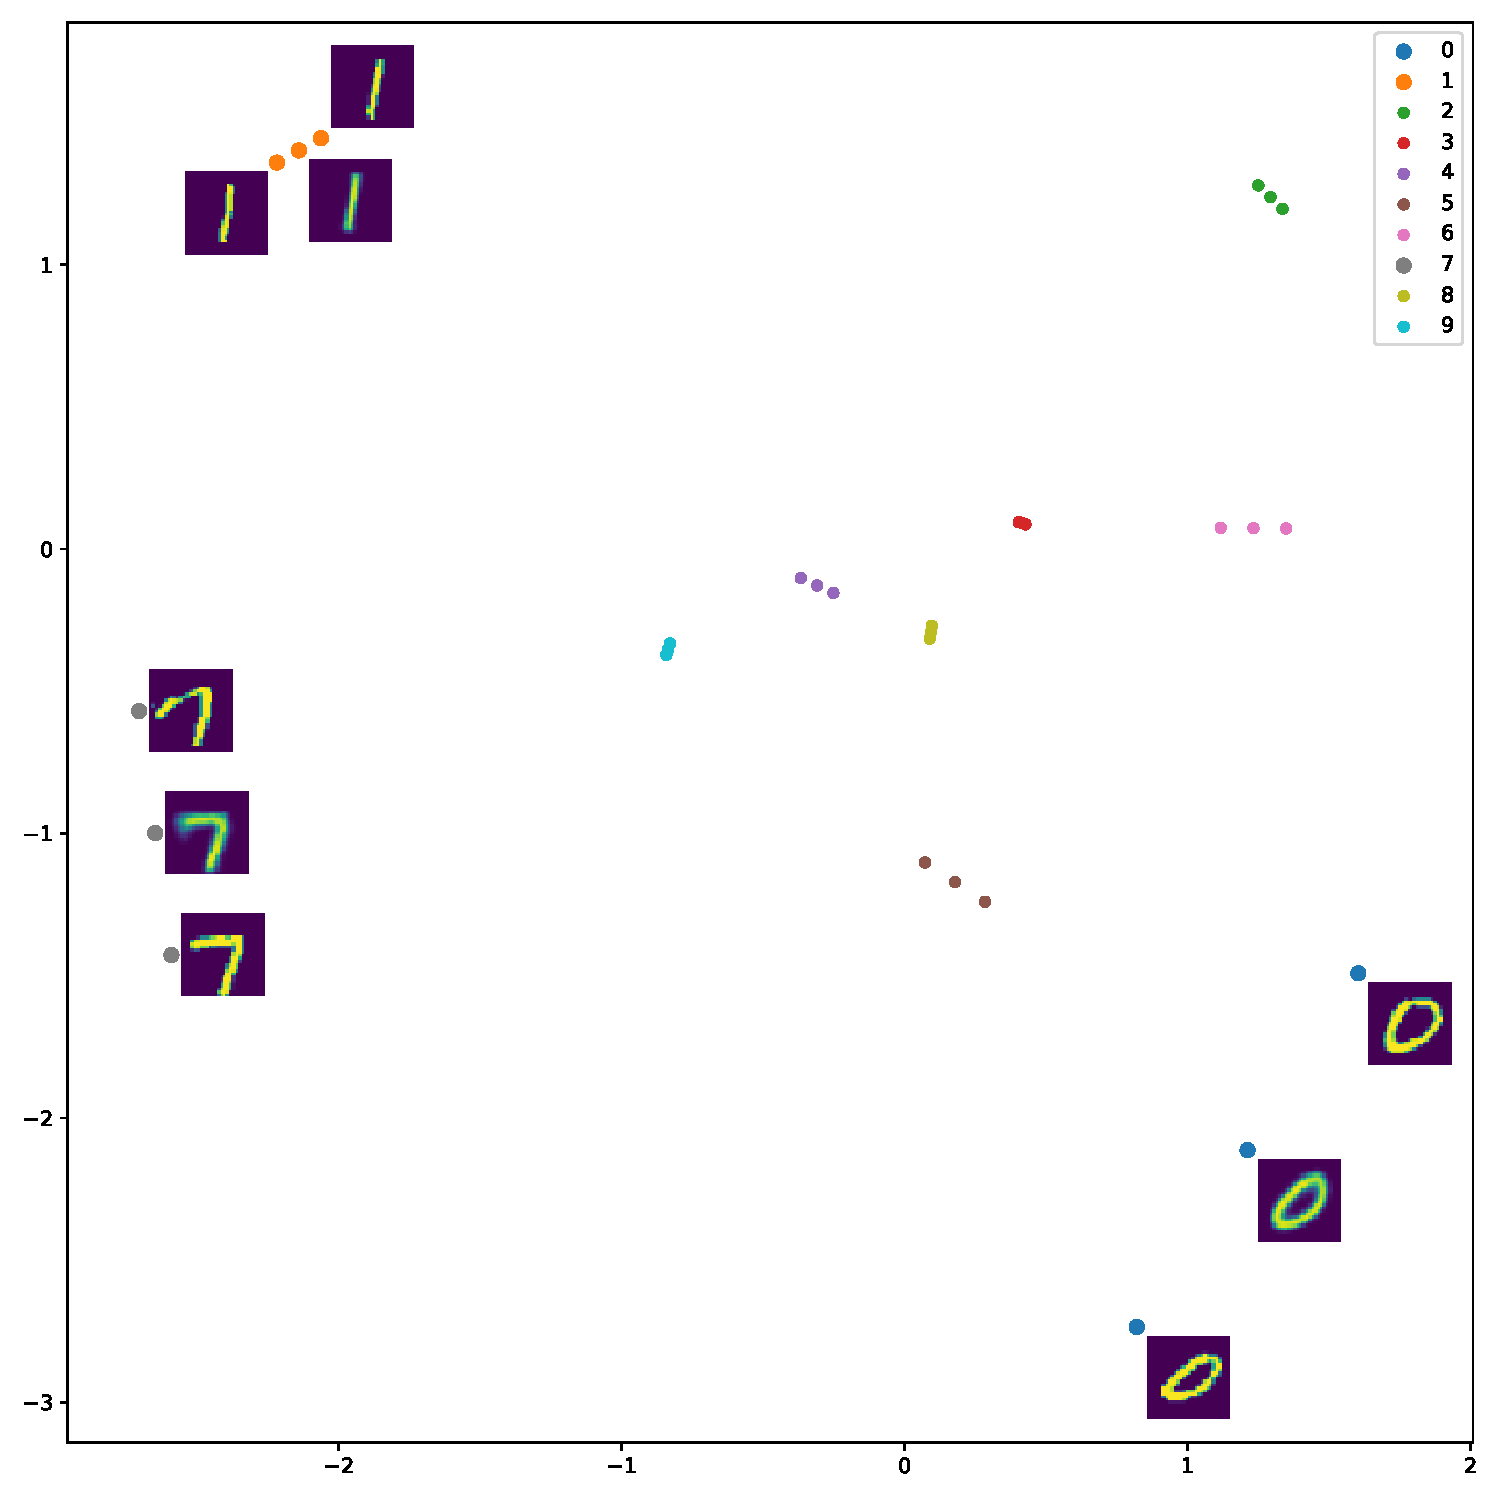
\includegraphics[width=\textwidth]{gfx/evaluation/feature_space/interpolation}
    \caption{Interpolation im Latent-Space}
  \end{figure}
\end{minipage}
\end{frame}

\begin{frame}{Sampling Methoden}
\begin{itemize}
  \item Sampling aus Normalverteilung
    \begin{equation*}
      \hat{z_i} \sim \mathcal{N}(0, \alpha)
    \end{equation*}
  \item Addition von Rauschen (Noise)
    \begin{equation*}
      \hat{z_i} = z_i + \epsilon, \epsilon \sim \mathcal{N}(0, \alpha)
    \end{equation*}
  \item Interpolation / Extrapolation zu k-Nächsten Nachbarn
    \begin{equation*}
      \hat{z_i} = \pm \alpha \cdot \left[\mu_\phi(x_k) - \mu_\phi(x_i)\right] + \mu_\phi(x_i)
    \end{equation*}
\end{itemize}
\end{frame}

\begin{frame}{Sampling Methoden}
\begin{itemize}
  \item Sampling aus Normalverteilung \hfill {\color{red}$\leftarrow$ \textbf{Wie werden Labels zugeordnet?}}
    \begin{equation*}
      \hat{z_i} \sim \mathcal{N}(0, \alpha)
    \end{equation*}
  \item Addition von Rauschen (Noise)
    \begin{equation*}
      \hat{z_i} = z_i + \epsilon, \epsilon \sim \mathcal{N}(0, \alpha)
    \end{equation*}
  \item Interpolation / Extrapolation zu k-Nächsten Nachbarn
    \begin{equation*}
      \hat{z_i} = \pm \alpha \cdot \left[\mu_\phi(x_k) - \mu_\phi(x_i)\right] + \mu_\phi(x_i)
    \end{equation*}
\end{itemize}
\end{frame}

\begin{frame}{Multi-VAE}
  \begin{minipage}[c]{.49\textwidth}
    \begin{figure}[hbt]
      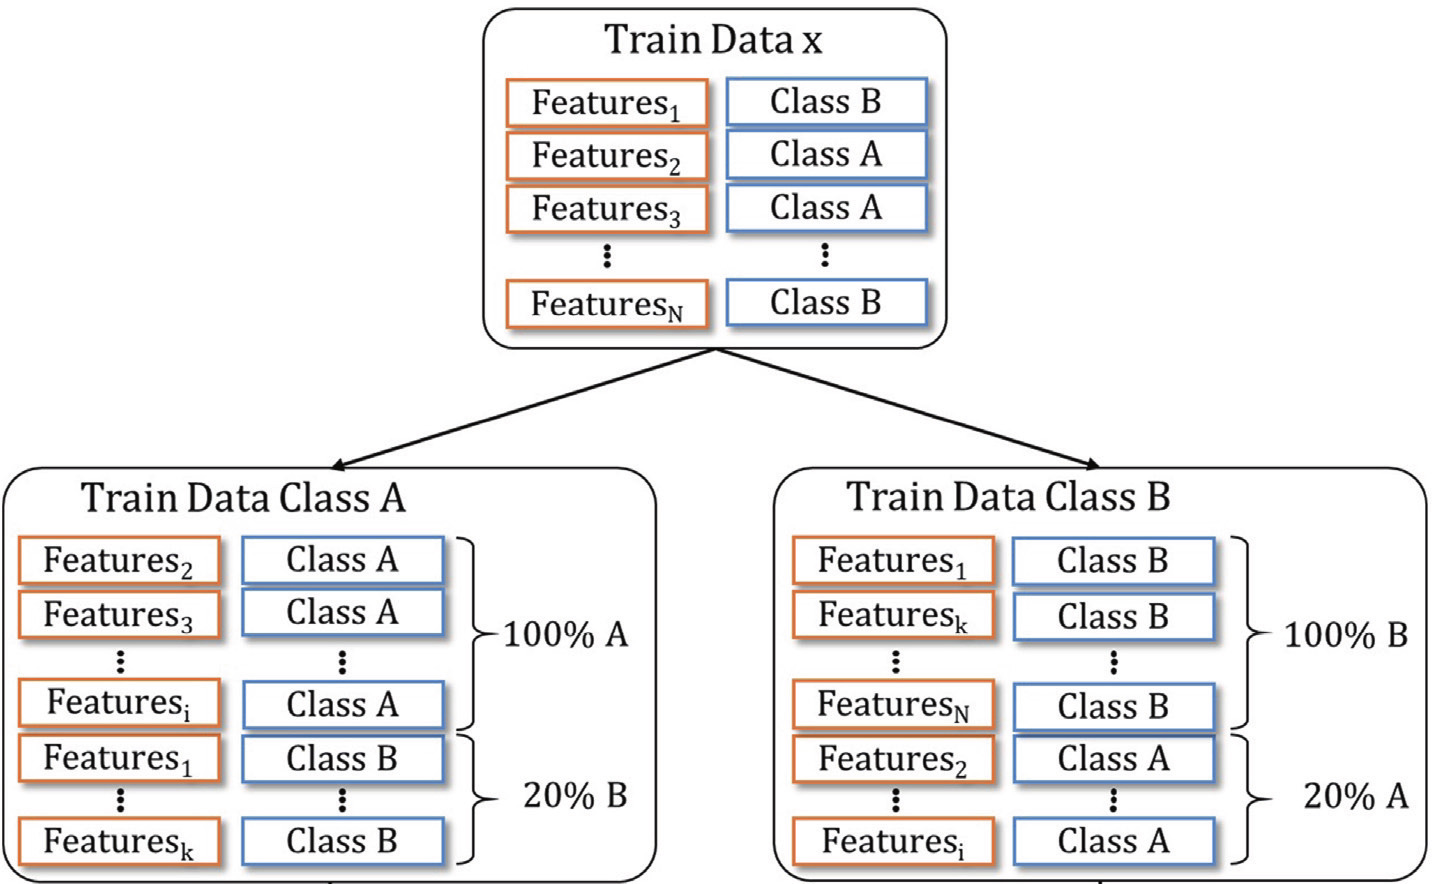
\includegraphics[width=\textwidth]{gfx/methodology/ds_split}
      \caption{Aufteilung des Datensatzes$^1$}
    \end{figure}
  \end{minipage}
  \begin{minipage}[c]{.5\textwidth}
    \begin{itemize}
      \item Trainiere einen VAE je Klasse
      \item Aufteilung des Datensatzes
      \item (optional) Mix-In der anderen Klassen zu 20\%
    \end{itemize}
  \end{minipage}
  \vfill
  {\tiny $^1$ entnommen aus \cite{Moreno-Barea2020}}
\end{frame}

\begin{frame}{Single- / Multi-VAE}
\begin{minipage}[c]{.50\textwidth}
  \center{\textbf{Single-VAE}}
\end{minipage}\hfill
\begin{minipage}[c]{.45\textwidth}
  \center{\textbf{Multi-VAE}}
\end{minipage}
\vfill
\begin{minipage}[c]{.50\textwidth}
  \begin{itemize}
    \item selbst-überwacht Trainierbar\\
      $\Rightarrow$ Nutzen großer Datenmengen
    \item Sampling hängt von Originalbeispielen ab
  \end{itemize}
\end{minipage}\hfill
\begin{minipage}[c]{.45\textwidth}
  \begin{itemize}
    \item Label Information benötigt
    \item Zufälliges Sampling möglich
    \item Erfasst Klassenmerkmale besser
  \end{itemize}
\end{minipage}
\end{frame}

\begin{frame}{Generative Classifier (GC)}
\centering
\begin{minipage}[c]{.8\textwidth}
  \begin{figure}[hbt]
  \centering
  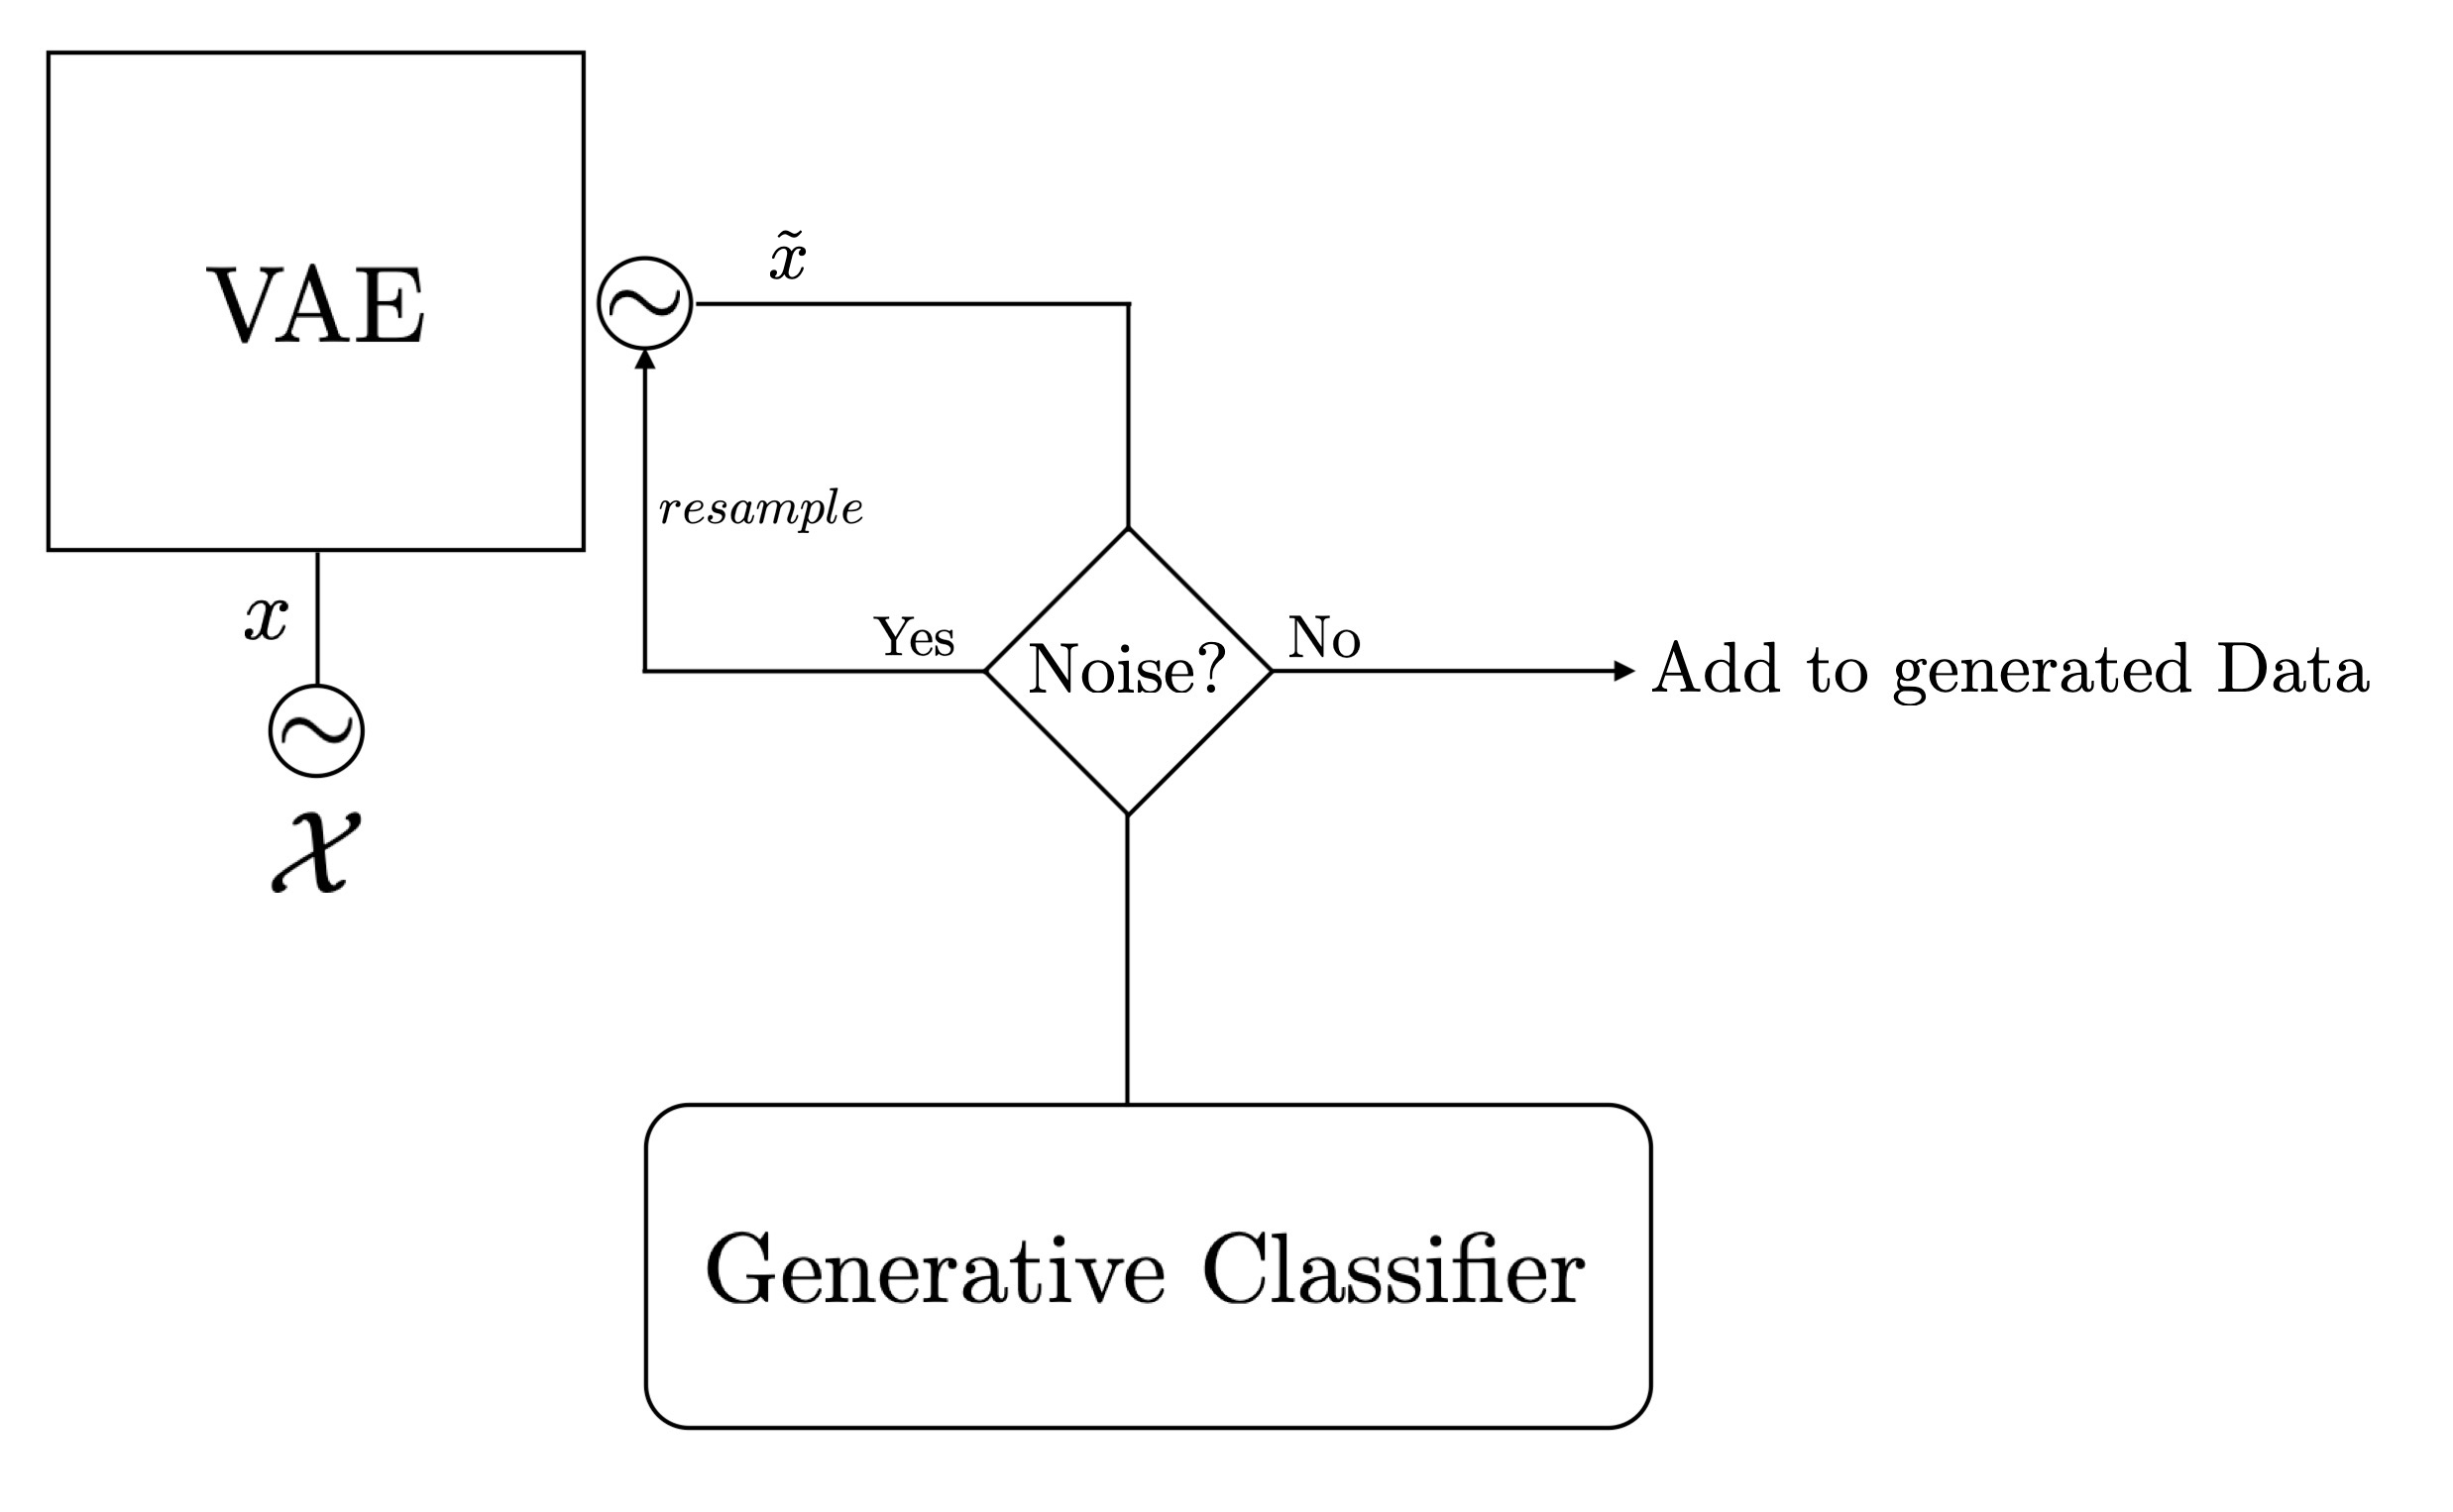
\includegraphics[width=\textwidth]{gfx/methodology/gc}
  \caption{Konzept: Generative Classifier}
  \end{figure}
\end{minipage}
\end{frame}

\begin{frame}{Generative Classifier - Training}
  \begin{itemize}
    \item Erzeugen verrauschter Originalbeispiele \,\, {\color{mDarkTeal} $\Rightarrow$ Für numerische Daten}
    \item Verwenden eines frühen VAE Modells, um ''schlechte'' Rekonstruktionen zu simulieren \,\,\,\, {\color{mDarkTeal} $\Rightarrow$ Für Bilddaten}
  \end{itemize}
  $\Rightarrow$ Zusätzliche Hyperparameter
\end{frame}


\section{Evaluation}
%\begin{frame}{Latent-Space}
%\begin{minipage}[c]{.5\textwidth}
%  \begin{figure}[hbt]
%  \centering
%  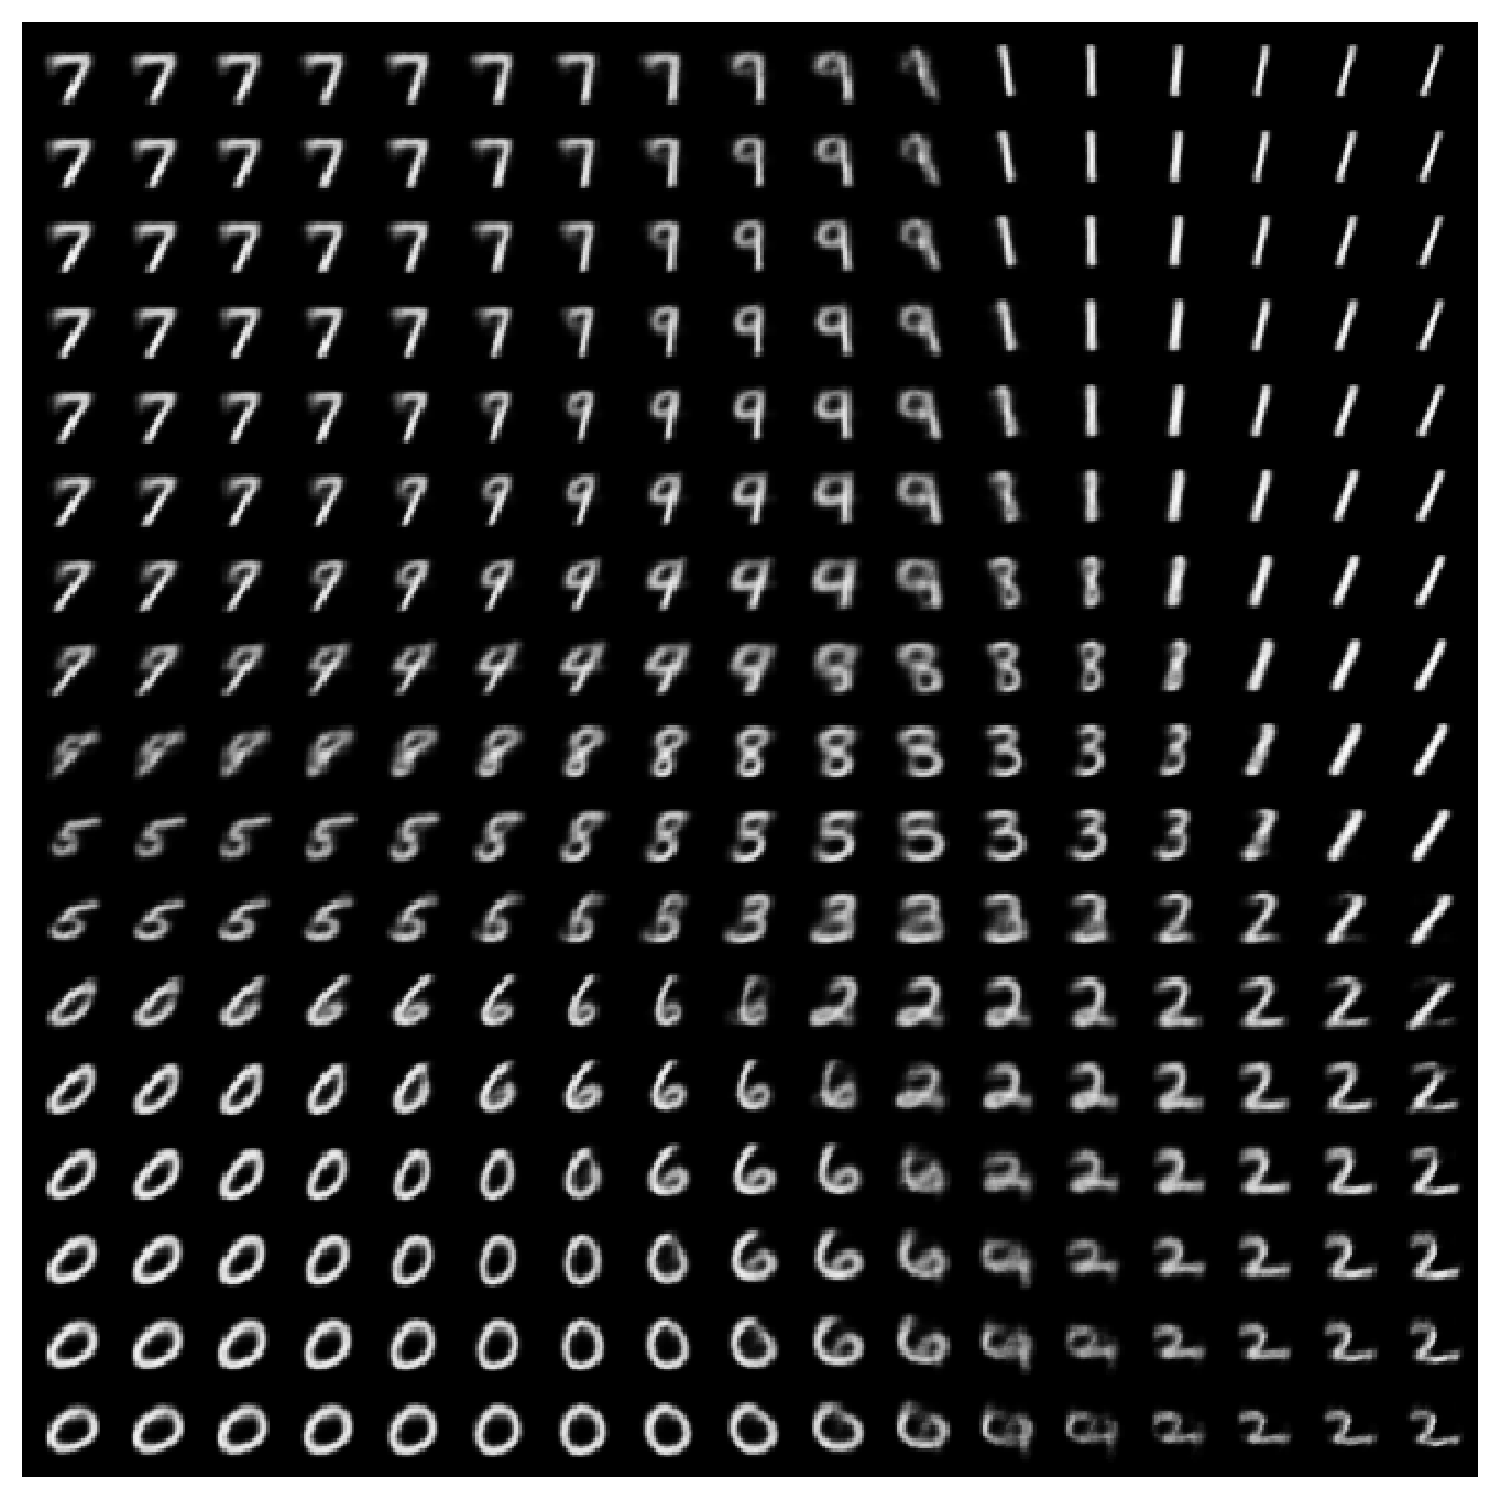
\includegraphics[width=\textwidth]{gfx/evaluation/feature_space/mnist_grid.pdf}
%  \caption{MNIST Rekonstruktionen}
%\end{figure}
%\end{minipage}
%\end{frame}

\begin{frame}{Latent-Space Clusterbildung}
  \begin{minipage}[c]{\textwidth}
    \begin{figure}[hbt]
    \centering
    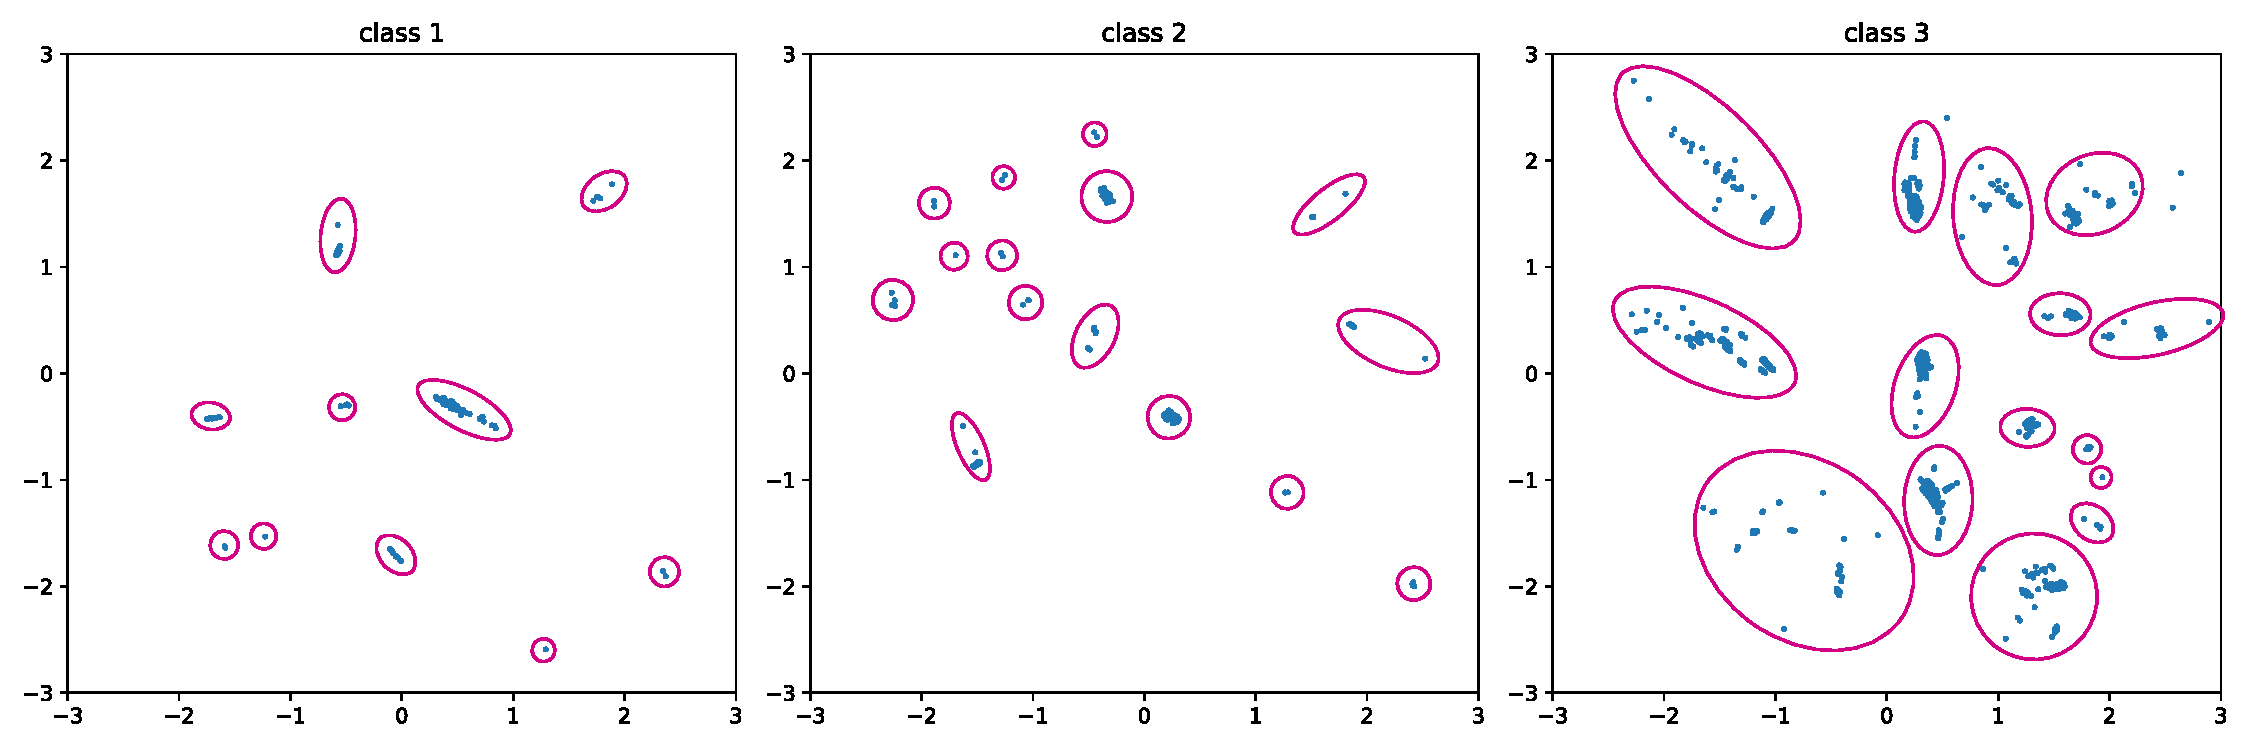
\includegraphics[width=\textwidth]{gfx/evaluation/feature_space/discrete_problem_with_cluster}
    \caption{Clusterbildung bei diskreten Attributen (Datensatz \textit{thyroid})}
    \end{figure}
  \end{minipage}
\end{frame}

\begin{frame}{PROBEN1 Performanz}
\begin{minipage}[c]{.49\textwidth}
  \begin{table}[hbt]
  \centering
  \scalebox{.55}{\begin{tabular}{l|c|c|c|c}
  \toprule
  Datensatz      & $\beta$             & Baseline & VAE            & VAE + GC       \\ \hline
  card           & norm=0.133          & 0.871    & 0.873          & 0.869          \\
  balance: Ja    & 0.5                 & 0.871    & 0.868          & 0.864          \\
  Mix data: Nein & \textbf{1.0}        & 0.871    & \textbf{0.876} & 0.871          \\ \midrule
  diabetes       & norm=0.25           & 0.823    & 0.831          & 0.826          \\
  balance: Ja    & 0.5                 & 0.823    & 0.830          & 0.822          \\
  Mix data: Nein & \textbf{1.0}        & 0.823    & 0.827          & \textbf{0.833} \\ \midrule
  geneN          & norm=0.033          & 0.813    & 0.802          & 0.814          \\
  balance: Nein  & \textbf{0.5}        & 0.813    & \textbf{0.818} & 0.813          \\
  Mix data: Ja   & 1.0                 & 0.813    & 0.812          & 0.813          \\ \midrule
  glass          & norm=0.222          & 0.985    & 0.977          & 0.985          \\
  balance: Ja    & 0.5                 & 0.985    & 0.977          & 0.985          \\
  Mix data: Nein & 1.0                 & 0.985    & 0.984          & 0.985          \\ \midrule
  horse          & \textbf{norm=0.1}   & 0.828    & 0.837          & \textbf{0.844} \\
  balance: Ja    & 0.5                 & 0.828    & 0.833          & 0.835          \\
  Mix data: Nein & 1.0                 & 0.828    & 0.836          & 0.828          \\ \midrule
  thyroid        & \textbf{norm=0.095} & 0.954    & 0.952          & \textbf{0.956} \\
  balance: Nein  & \textbf{0.5}        & 0.954    & 0.927          & \textbf{0.956} \\
  Mix data: Ja   & 1.0                 & 0.954    & 0.925          & 0.954          \\
  \bottomrule
  \end{tabular}}
  \caption{PROBEN1 Weighted-F1-Score}
  \end{table}
  \end{minipage}
  \hfill
  \begin{minipage}[c]{.45\textwidth}
    \begin{itemize}
      \item Sampling aus $\mathcal{N}(0, I)$
      \item $\sim 6000$ Schritte (VAE)
      \item Latent-Space Dimension $d = 2$
    \end{itemize}
  \end{minipage}
\end{frame}

\begin{frame}{PROBEN1 Few-Shot Szenario}
\begin{minipage}[c]{.5\textwidth}
  \begin{table}[hbt]
  \centering
  \scalebox{.55}{\begin{tabular}{l|c|c|c|c}
  \toprule
  \begin{tabular}[c]{@{}l@{}}\# Beispiele\\ pro Klasse\end{tabular} & \begin{tabular}[c]{@{}l@{}}\# Generierte\\ Beispiele\end{tabular} & Baseline       & VAE            & VAE + GC       \\ \hline
5                                                                 & 5                                                                 & 0.619          & \textbf{0.693} & 0.675          \\
10                                                                & 10                                                                & 0.727          & \textbf{0.778} & 0.761          \\
20                                                                & 20                                                                & 0.735          & 0.753          & \textbf{0.778} \\
30                                                                & 30                                                                & 0.772          & 0.786          & \textbf{0.796} \\
50                                                                & 50                                                                & \textbf{0.818} & 0.815          & 0.808          \\
100                                                               & 100                                                               & \textbf{0.935} & 0.927          & 0.922          \\
  \bottomrule
  \end{tabular}}
  \caption{\textit{thyroid} Weighted-F1-Score}
  \end{table}
  \vspace*{-1.2\baselineskip}
  \begin{figure}[hbt]
  \centering
  \scalebox{.7}{\begin{tikzpicture}
  \begin{axis}
  [
    width=1.5\textwidth,
    height = 4cm,
    symbolic x coords={5,10,20,30,50,100},
    xtick={5,10,20,30,50,100},
    xlabel={\# Beispiele pro Klasse}, 
    ylabel={$\Delta$ F-Score}, 
    grid,
    legend pos=south west,
  ]

  \addplot[blue, mark=* , solid] table[col sep=comma, x=n_originals, y=improvement]{data/evaluation/thyroid-few-shot.csv};
  \addlegendentry{F1-Increase}

  \end{axis}
  \end{tikzpicture}}
  \caption{F1 Verbesserung}
  \end{figure}
  \end{minipage}
  \hfill
  \begin{minipage}[c]{.45\textwidth}
    \begin{itemize}
      \item Reduzierte Datensatzgröße
      \item Verbesserung nimmt mit mehr Daten ab
    \end{itemize}
  \end{minipage}
\end{frame}

\begin{frame}{MNIST Few-Shot Szenario}
Latent-Space Dimension $d = 50$, $\beta = 0.5$, keine $\beta$-Normalisierung
  \begin{table}[hbt]
\centering
\scalebox{.55}{\begin{tabular}{l|c|c|c|c|c|c|c}
\toprule
\begin{tabular}[c]{@{}l@{}}\# Beispiele\\ pro Klasse\end{tabular} & Baseline       & Noise & Interpolation  & Extrapolation  & \begin{tabular}[c]{@{}c@{}}Interpolation\\ + Noise\end{tabular} & \begin{tabular}[c]{@{}c@{}}Extrapolation\\ + Noise\end{tabular} & Multi-VAE      \\ \hline
2                                                                 & 0.660          & 0.619 & 0.669          & 0.654          & 0.674                                                           & 0.653                                                           & \textbf{0.678} \\
3                                                                 & 0.699          & 0.662 & \textbf{0.706} & 0.700          & 0.703                                                           & \textbf{0.706}                                                  & \textbf{0.706} \\
4                                                                 & 0.734          & 0.703 & 0.740          & 0.732          & \textbf{0.744}                                                  & 0.734                                                           & 0.734          \\
5                                                                 & 0.776          & 0.721 & 0.782          & 0.756          & \textbf{0.787}                                                  & 0.768                                                           & 0.770          \\
10                                                                & 0.849          & 0.825 & 0.855          & \textbf{0.861} & 0.859                                                           & 0.849                                                           & 0.854          \\
20                                                                & 0.905          & 0.878 & 0.905          & \textbf{0.911} & 0.905                                                           & 0.909                                                           & 0.904          \\
30                                                                & 0.929          & 0.898 & 0.924          & \textbf{0.930} & 0.927                                                           & 0.923                                                           & 0.923          \\
50                                                                & 0.941          & 0.920 & 0.939          & 0.941          & \textbf{0.942}                                                  & 0.938                                                           & 0.937          \\
100                                                               & \textbf{0.954} & 0.940 & 0.951          & 0.953          & 0.951                                                           & 0.950                                                           & 0.949          \\
200                                                               & \textbf{0.962} & 0.950 & 0.958          & 0.960          & 0.956                                                           & 0.958                                                           & 0.956          \\
500                                                               & \textbf{0.964} & 0.955 & 0.962          & 0.963          & 0.962                                                           & 0.963                                                           & 0.959          \\
1000                                                              & \textbf{0.965} & 0.952 & 0.963          & 0.964          & 0.964                                                           & 0.963                                                           & 0.960          \\
2000                                                              & \textbf{0.967} & 0.953 & 0.964          & 0.966          & 0.963                                                           & 0.964                                                           & 0.963          \\
\bottomrule
\end{tabular}}
\caption{MNIST Few-Shot: Weighted-F1-Score}
\end{table}
\end{frame}

\begin{frame}{MNIST - Nur generierte Daten}
Latent-Space Dimension $d = 50$, $\beta = 0.5$, keine $\beta$-Normalisierung\\
\# Originalbeispiele = 5
  \begin{table}[hbt]
\centering
\scalebox{.55}{\begin{tabular}{l|c|c|c|c|c}
\toprule
\begin{tabular}[c]{@{}l@{}}\# Generierte Beispiele\\ pro Klasse\end{tabular} & Baseline & Noise & \begin{tabular}[c]{@{}c@{}}Interpolation\\ + Noise\end{tabular} & \begin{tabular}[c]{@{}c@{}}Extrapolation\\ + Noise\end{tabular} & Multi-VAE      \\ \hline
2                                                                            & 0.776    & 0.402 & \textbf{0.636}                                                  & 0.542                                                           & 0.635          \\
3                                                                            & 0.776    & 0.518 & \textbf{0.681}                                                  & 0.637                                                           & 0.666          \\
4                                                                            & 0.776    & 0.542 & \textbf{0.699}                                                  & 0.616                                                           & 0.697          \\
5                                                                            & 0.776    & 0.555 & 0.686                                                           & 0.574                                                           & \textbf{0.712} \\
10                                                                           & 0.776    & 0.618 & 0.740                                                           & 0.696                                                           & \textbf{0.764} \\
20                                                                           & 0.776    & 0.670 & 0.748                                                           & 0.740                                                           & \textbf{0.773} \\
30                                                                           & 0.776    & 0.700 & 0.765                                                           & 0.744                                                           & \textbf{0.769} \\
50                                                                           & 0.776    & 0.726 & \textbf{0.774}                                                  & 0.754                                                           & 0.763          \\
100                                                                          & 0.776    & 0.750 & \textbf{0.797}                                                  & 0.771                                                           & 0.768          \\
200                                                                          & 0.776    & 0.765 & \textbf{0.790}                                                  & 0.761                                                           & 0.771          \\
500                                                                          & 0.776    & 0.788 & \textbf{0.792}                                                  & 0.770                                                           & 0.774          \\
1000                                                                         & 0.776    & 0.775 & \textbf{0.788}                                                  & 0.773                                                           & 0.767          \\
2000                                                                         & 0.776    & 0.777 & \textbf{0.792}                                                  & 0.765                                                           & 0.770          \\
\bottomrule
\end{tabular}}
\caption{Weighted-F1-Score bei nur generierten Daten}
\end{table}
\end{frame}

\begin{frame}{MNIST - Nur generierte Daten}
\begin{minipage}[c]{\textwidth}
\begin{figure}[hbt]
\centering
\scalebox{.6}{\begin{tikzpicture}
\begin{axis}
[
  width=1.2\textwidth,
  height=5cm,
  symbolic x coords={2,3,4,5,10,20,30,50,100,200,500,1000,2000},
  xtick={2,3,4,5,10,20,30,50,100,200,500,1000,2000},
  xlabel={Generierte Beispiele pro Klasse}, 
  ylabel={F1 Score}, 
  grid,
  legend pos=south east,
]

\addplot[blue, no marks, solid] table[col sep=comma, x=n_generated, y=baseline]{data/evaluation/MNIST-GEN*-5.csv};
\addlegendentry{Baseline}

\addplot[red, no marks, solid] table[col sep=comma, x=n_generated, y=interpolation_noise]{data/evaluation/MNIST-GEN*-5.csv};
\addlegendentry{Interpolation + Noise}

\addplot[violet, no marks, solid] table[col sep=comma, x=n_generated, y=multi_vae]{data/evaluation/MNIST-GEN*-5.csv};
\addlegendentry{Multi-VAE}

\end{axis}
\end{tikzpicture}}
\caption{Weighted-F1-Score bei nur generierten Daten}
\end{figure}
\end{minipage}
\end{frame}

\begin{frame}{MNIST Few-Shot: Mehr generierte Daten}
Latent-Space Dimension $d = 50$, $\beta = 0.5$, keine $\beta$-Normalisierung\\
\# Generierte Beispiele pro Klasse = 2000
  \begin{table}[hbt]
\centering
\scalebox{.55}{\begin{tabular}{l|c|c|c|c|c}
\toprule
\begin{tabular}[c]{@{}l@{}}\# Beispiele\\ pro Klasse\end{tabular} & Baseline       & Noise          & \begin{tabular}[c]{@{}c@{}}Interpolation\\ + Noise\end{tabular} & \begin{tabular}[c]{@{}c@{}}Extrapolation\\ + Noise\end{tabular} & Multi-VAE \\ \hline
2                                                                 & 0.660          & \textbf{0.679} & 0.668                                                           & 0.638                                                           & 0.634     \\
3                                                                 & 0.699          & \textbf{0.716} & 0.715                                                           & 0.711                                                           & 0.687     \\
4                                                                 & 0.734          & \textbf{0.748} & 0.747                                                           & 0.740                                                           & 0.724     \\
5                                                                 & 0.776          & 0.779          & \textbf{0.795}                                                  & 0.772                                                           & 0.768     \\
10                                                                & 0.849          & 0.851          & 0.868                                                           & \textbf{0.871}                                                  & 0.839     \\
20                                                                & 0.905          & 0.894          & 0.907                                                           & \textbf{0.919}                                                  & 0.897     \\
30                                                                & 0.929          & 0.905          & 0.922                                                           & \textbf{0.936}                                                  & 0.916     \\
50                                                                & 0.941          & 0.914          & 0.935                                                           & \textbf{0.945}                                                  & 0.925     \\
100                                                               & \textbf{0.954} & 0.923          & 0.946                                                           & 0.951                                                           & 0.936     \\
200                                                               & \textbf{0.962} & 0.929          & 0.952                                                           & 0.960                                                           & 0.934     \\
500                                                               & \textbf{0.964} & 0.939          & 0.957                                                           & 0.960                                                           & 0.924     \\
1000                                                              & \textbf{0.965} & 0.946          & 0.960                                                           & 0.961                                                           & 0.913     \\
2000                                                              & \textbf{0.967} & 0.953          & 0.963                                                           & 0.964                                                           & 0.905     \\
\bottomrule
\end{tabular}}
\caption{MNIST Few-Shot: Weighted-F1-Score}
\end{table}
\end{frame}

\begin{frame}{Einfluss des $\beta$-Faktors}
\centering
\begin{minipage}[c]{\textwidth}
\centering
  \begin{figure}[hbt]
\centering
\begin{subfigure}{.24\textwidth}
  \centering
  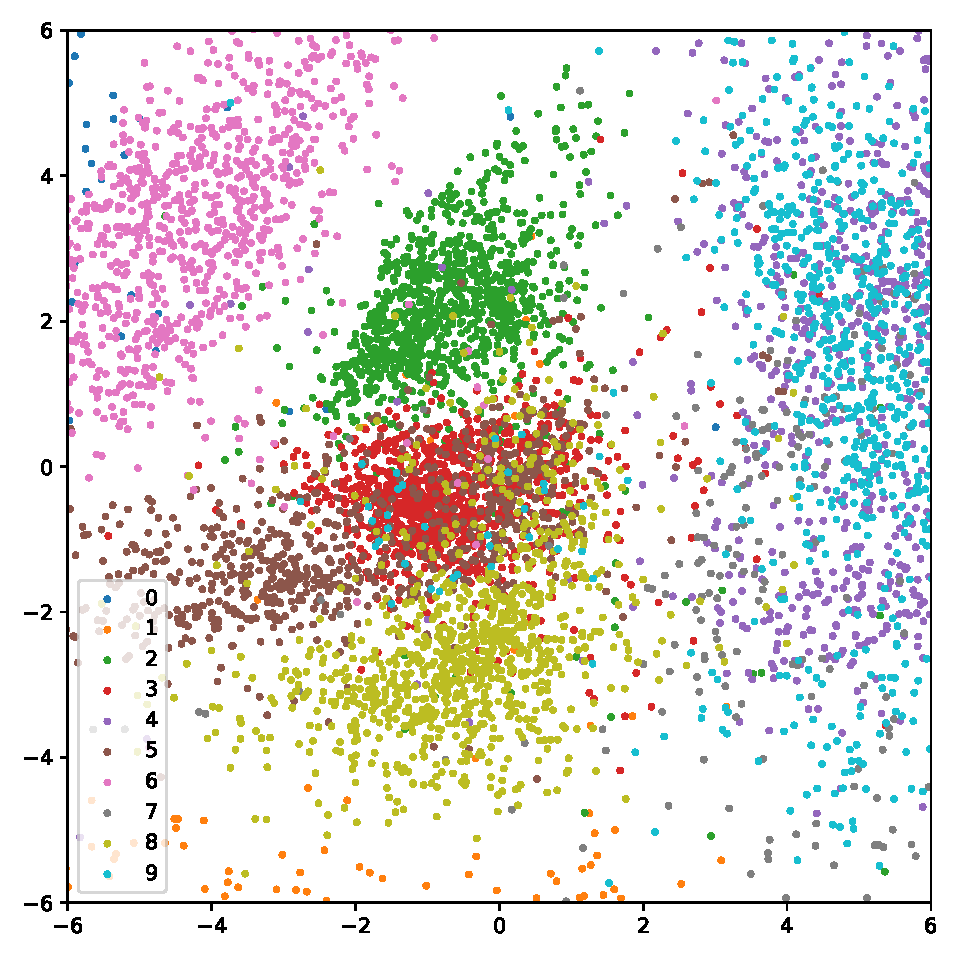
\includegraphics[width=\textwidth]{gfx/evaluation/feature_space/beta=0.001.pdf}
  \caption{$\beta = 0.001$}
\end{subfigure}
\begin{subfigure}{.24\textwidth}
  \centering
  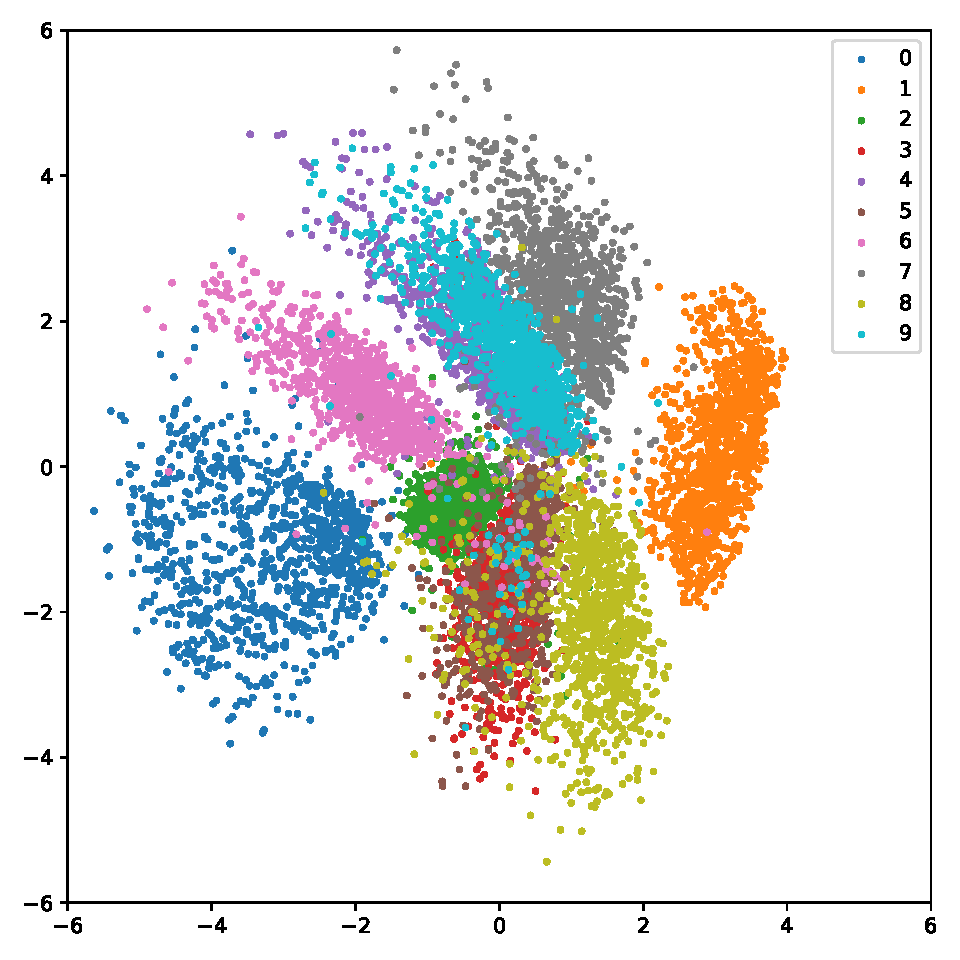
\includegraphics[width=\textwidth]{gfx/evaluation/feature_space/beta=0.1.pdf}
  \caption{$\beta = 0.1$}
\end{subfigure}
\begin{subfigure}{.24\textwidth}
  \centering
  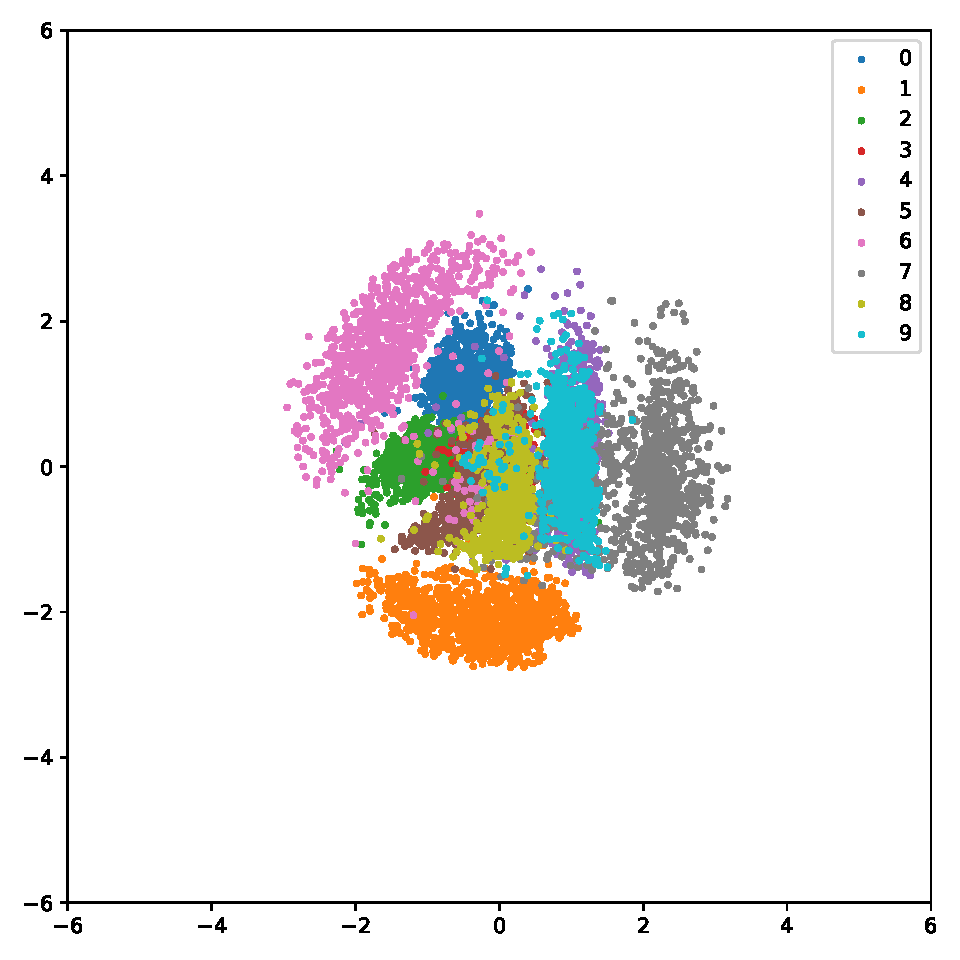
\includegraphics[width=\textwidth]{gfx/evaluation/feature_space/beta=1.0.pdf}
  \caption{$\beta = 1.0$}
\end{subfigure}
\begin{subfigure}{.24\textwidth}
  \centering
  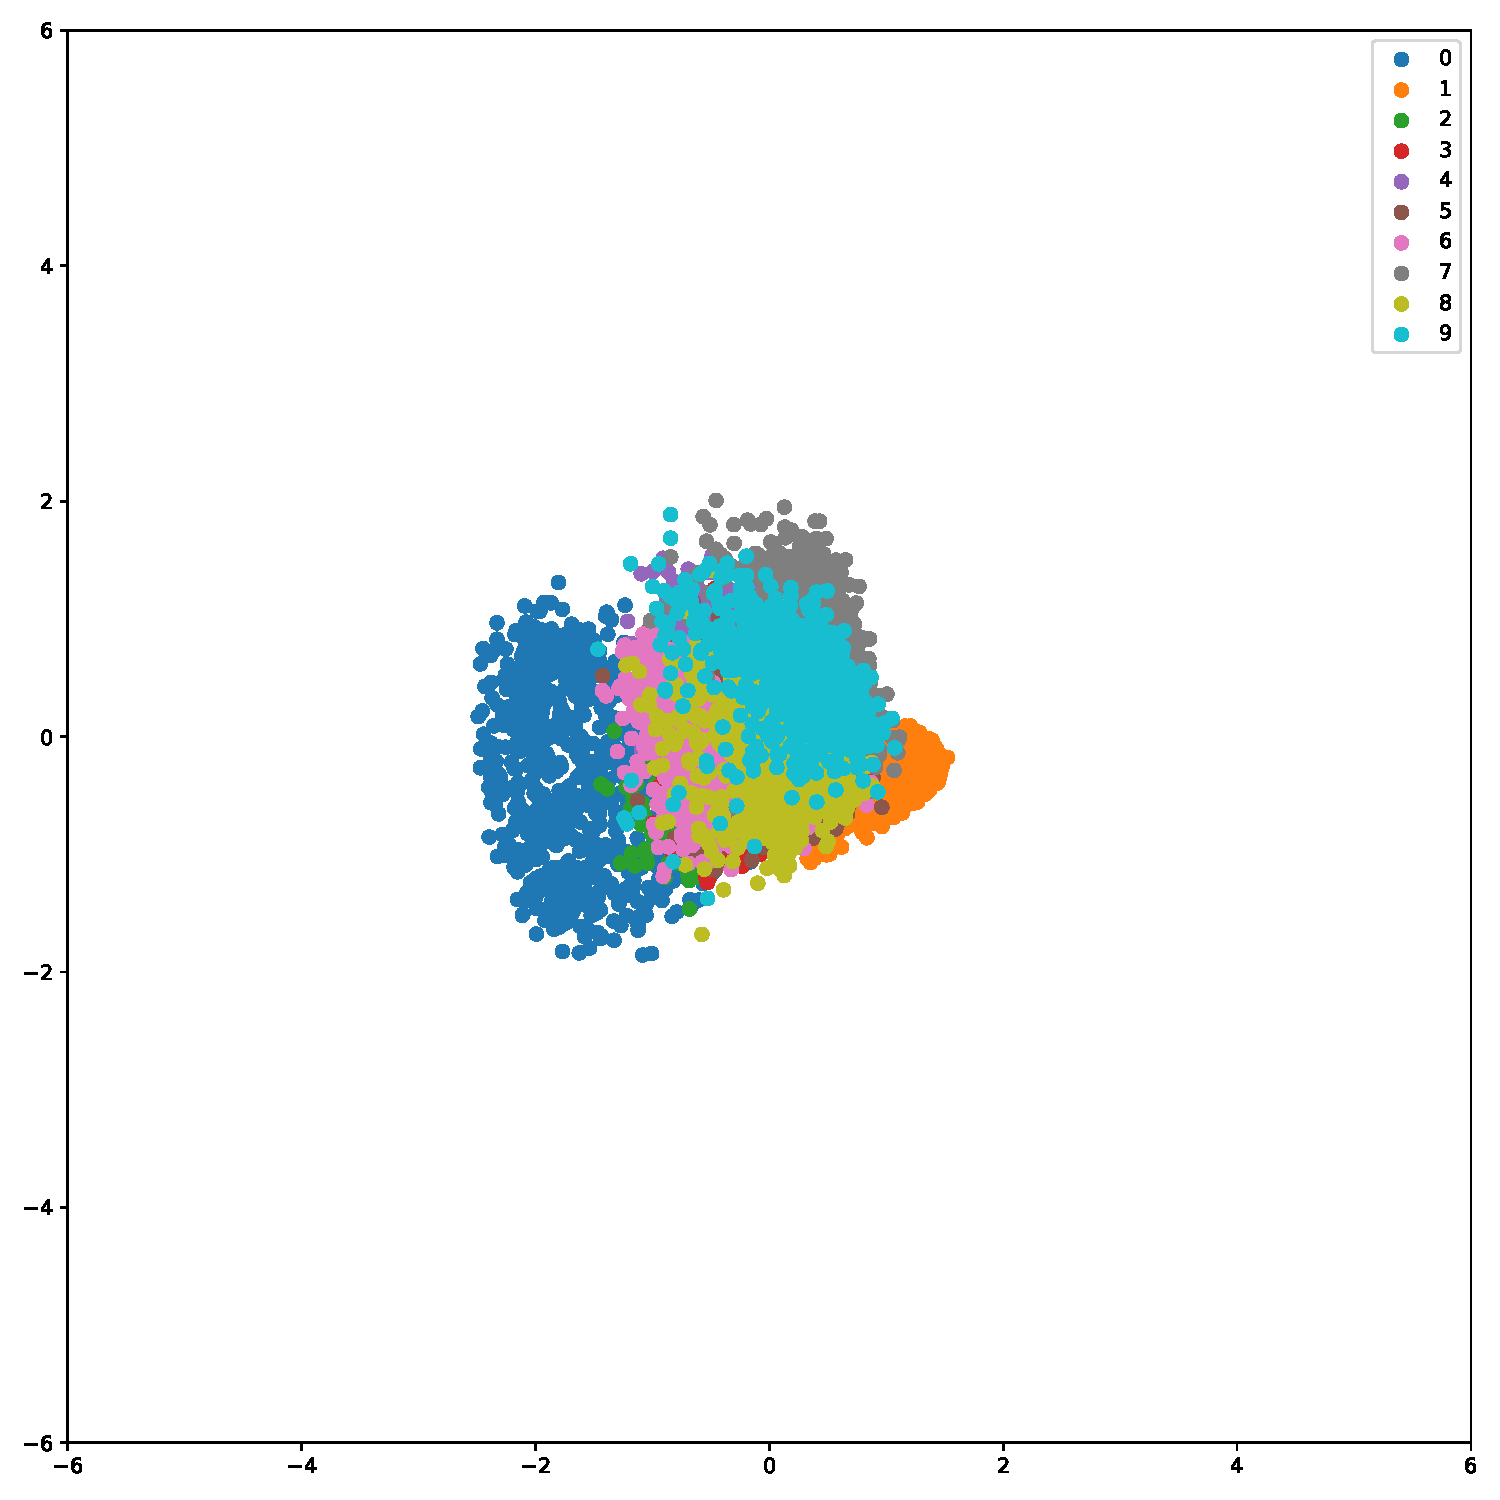
\includegraphics[width=\textwidth]{gfx/evaluation/feature_space/beta=10.0.pdf}
  \caption{$\beta = 10.0$}
\end{subfigure}
\caption{Latent-Space MNIST mit verschiedenen Werten für $\beta$}
\end{figure}
\end{minipage}
\begin{itemize}
  \item Hohe $\beta$-Werte führen zu unscharfen Rekonstruktionen
\end{itemize}
\end{frame}

\begin{frame}{$\beta$-VAE Disentanglement}
\centering
\begin{minipage}[c]{\textwidth}
  \begin{figure}[hbt]
  \centering
  \begin{subfigure}{\textwidth}
    \centering
    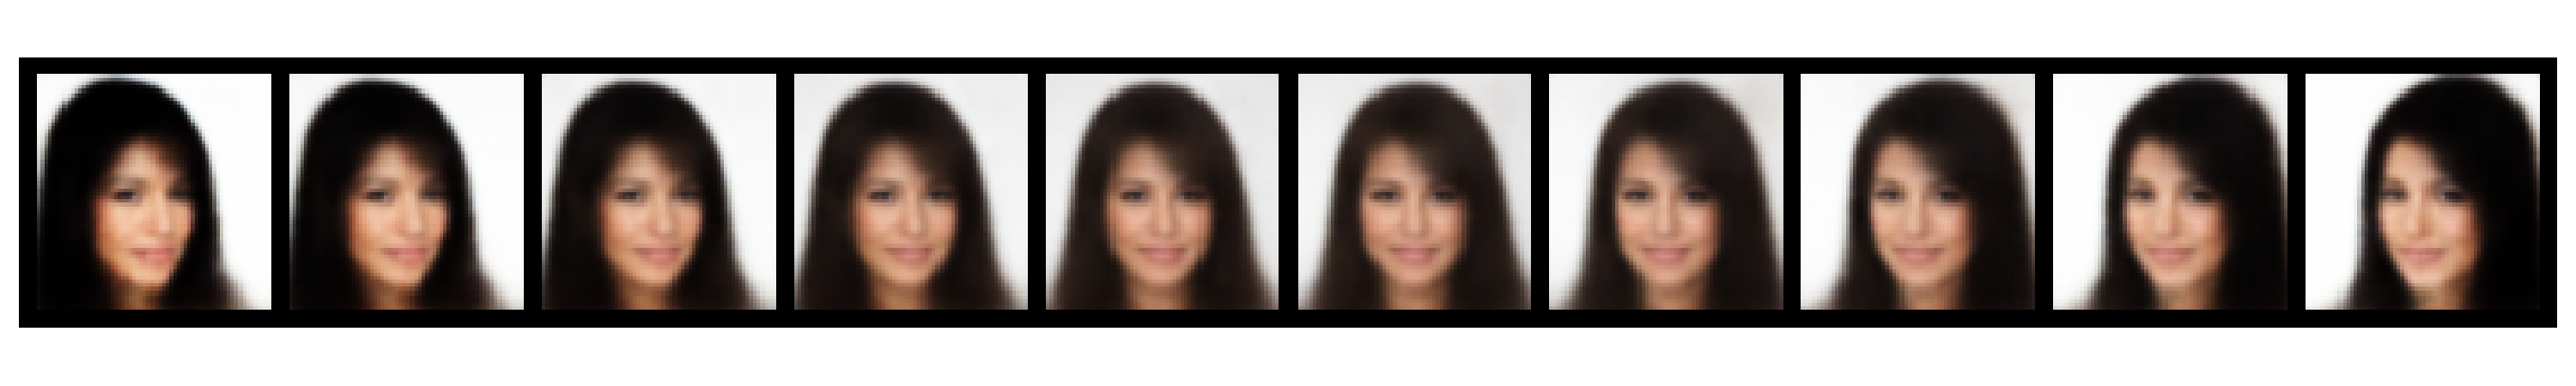
\includegraphics[width=\textwidth]{gfx/evaluation/celeba/CelebA-Rotation_1}
    \caption{$\beta = 150$}
  \end{subfigure}
  \begin{subfigure}{\textwidth}
    \centering
    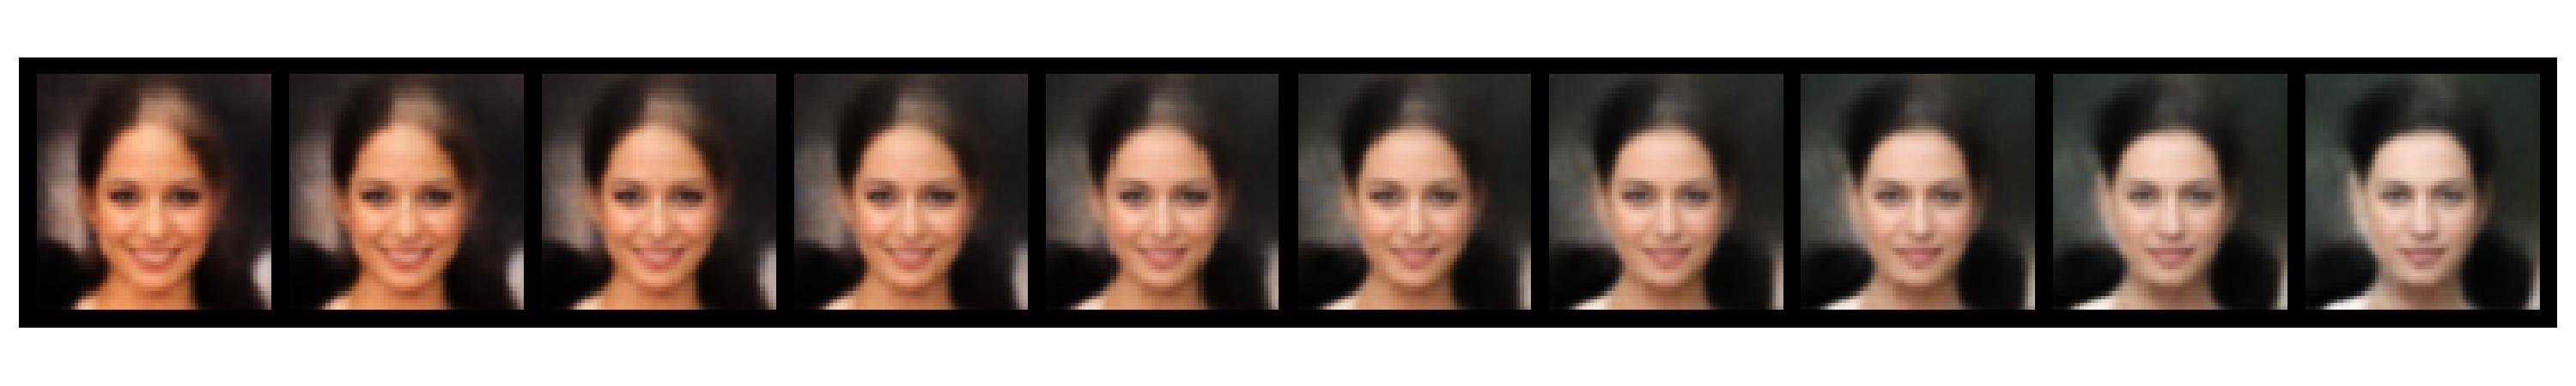
\includegraphics[width=\textwidth]{gfx/evaluation/celeba/regular-face-color}
    \caption{$\beta = 1$}
  \end{subfigure}
  \caption{Dimension Sweep CelebA; Trainiert mit $\beta_{norm}$}
  \end{figure}
\end{minipage}
\end{frame}

\begin{frame}{Limitationen von VAE}
  \begin{figure}[H]
  \centering
  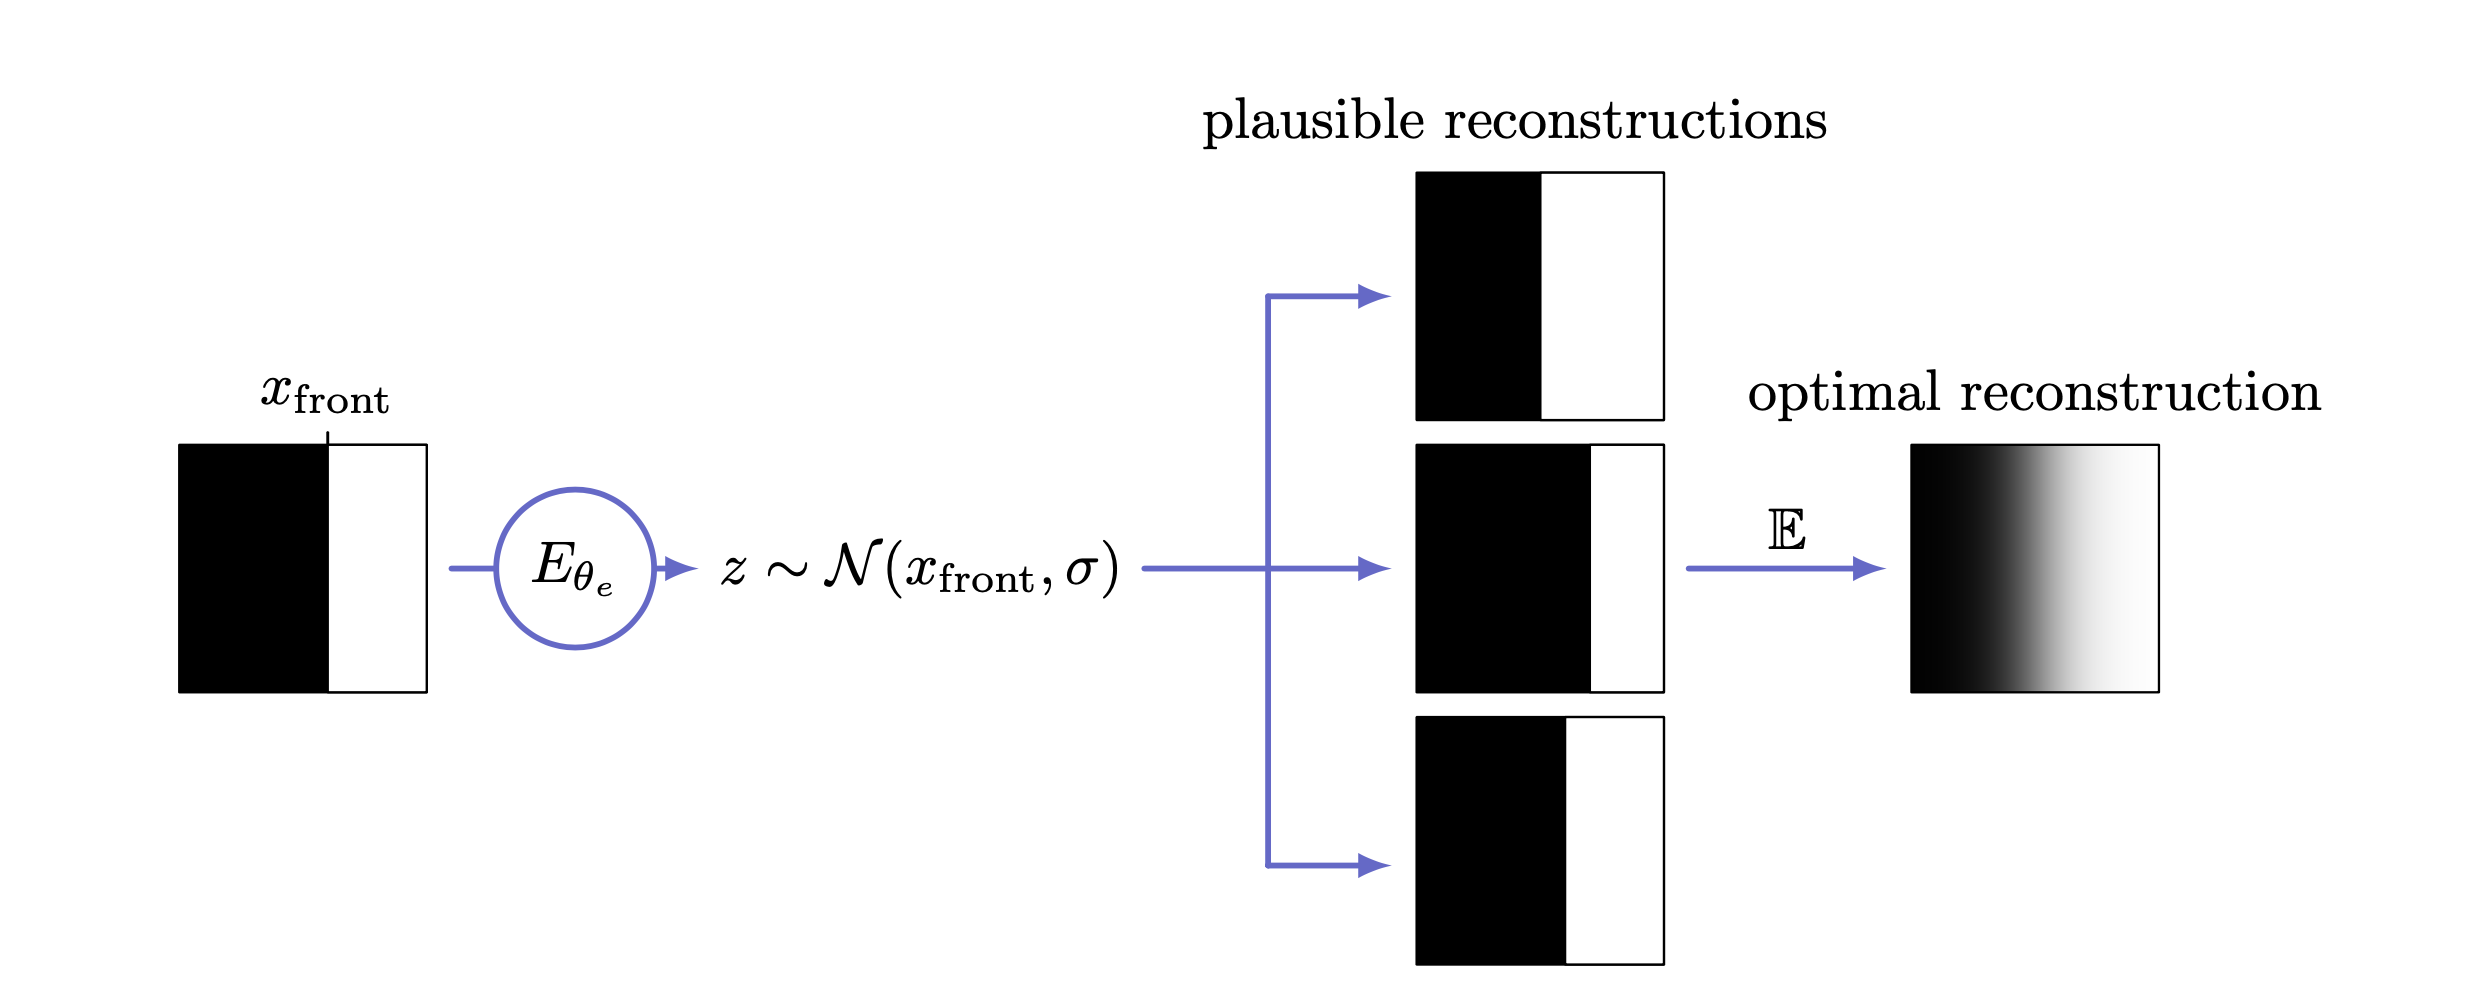
\includegraphics[width=.8\textwidth]{gfx/evaluation/recon_blur}
  \caption{Unschärfe Auftreten beim VAE$^1$}
  \label{fig:blur_explained}
\end{figure}
\vfill
{\tiny $^1$ entnommen aus \cite{Plumerault2020}}
\end{frame}


\section{Fazit}
\begin{frame}{Fazit}
  \textbf{Numerische Daten} (PROBEN1):
  \begin{itemize}
    \item Auf numerischen Daten Hyperparameter sensitiv, besonders bei diskreten Attributen
    \item Geringe Verbesserung der Klassifikations Güte
    \item Im Vergleich zu \cite{Moreno-Barea2020} (GAN) geringere Performanz
    \item Few-Shot kleine, konsistente Verbesserung
  \end{itemize}
\end{frame}

\begin{frame}{Fazit}
  \textbf{Bilddaten} (MNIST, CelebA):
  \begin{itemize}
    \item Nützliche Latent-Space Struktur
    \item Dekorrelation unabhängiger Merkmale ($\beta$-VAE)
    \item Few-Shot: Konsistente Verbesserung
    \item Single-VAE > Multi-VAE durch selbst-überwachtes Lernen
    \item Starke Unschärfe Effekte
  \end{itemize}
\end{frame}


\begin{frame}{Quellen}
    \AtNextBibliography{\tiny}
    \printbibliography
\end{frame}

% Begin of workaround: Hide the logo on plain slide
\begingroup
\setbeamertemplate{footline}{}
\plain{Fragen?}
\endgroup
% end of workaround

\end{document}
